\documentclass[sigplan,10pt,review,anonymous]{acmart}
\settopmatter{printfolios=true,printccs=false,printacmref=false}
\acmConference[PL'18]{ACM SIGPLAN Conference on Programming Languages}{January 01--03, 2018}{New York, NY, USA}
\acmYear{2018}
\acmISBN{} 
\acmDOI{} 
\startPage{1}
\setcopyright{none}
\bibliographystyle{ACM-Reference-Format}

\usepackage{booktabs}  
\usepackage{subcaption} 
\usepackage{amssymb}
\usepackage{stmaryrd}
\usepackage{bbm}
\usepackage{wrapfig}
\usepackage[greek,english]{babel}
\usepackage{ucs}
\usepackage[utf8x]{inputenc}
\usepackage{autofe}
\usepackage[references]{agda} 
\usepackage{newunicodechar}
\usepackage[nocenter]{qtree}
\usepackage{multicol}  
\usepackage{bbold}
\usepackage{tikz}
\usetikzlibrary{cd}
\usetikzlibrary{quotes}

\usepackage{tikzit}
\documentclass{llncs}
\usepackage{url}
\usepackage{proof}
\usepackage{amssymb}
\usepackage{stmaryrd}
\usepackage{listings}
\usepackage{graphicx}
\usepackage{comment}

\newcommand{\dgm}[2][1.5]{
\begin{center}
\scalebox{#1}{
\includegraphics{diagrams/#2.pdf}
}
\end{center}
}

\newcommand{\todo}[1]{\textbf{TODO:} #1}
\newcommand{\jacques}[1]{\textsc{Jacques says:} #1}
\newcommand{\amr}[1]{\textsc{Amr says:} #1}

\newcommand{\roshan}[1]{} 
%% \newcommand{\roshan}[1]{\textsc{Roshan says:} 
%%   \textit{#1}
%% }

\hyphenation{a-reas}

%subcode-inline{bnf-inline} name Pi
%! swap+ = \mathit{swap}^+
%! swap* = \mathit{swap}^*
%! dagger =  ^{\dagger}
%! assocl+ = \mathit{assocl}^+
%! assocr+ = \mathit{assocr}^+
%! assocl* = \mathit{assocl}^*
%! assocr* = \mathit{assocr}^*
%! identr* = \mathit{uniti}
%! identl* = \mathit{unite}
%! dist = \mathit{distrib}
%! factor = \mathit{factor}
%! (o) = \fatsemi
%! (;) = \fatsemi
%! (*) = \times
%! (+) = +
%! foldB = fold_B
%! unfoldB = unfold_B
%! foldN = fold_N
%! unfoldN = unfold_N
%! trace+ = \mathit{trace}^{+}
%! trace* = \mathit{trace}^{\times}
%! :-* = \multimap
%! :-+ = \multimap^{+}
%! emptyset = \emptyset

%subcode-inline{bnf-inline} regex \{\{(((\}[^\}])|[^\}])*)\}\} name main include Pi
%! [^ = \ulcorner
%! ^] = \urcorner
%! [v = \llcorner
%! v] = \lrcorner
%! [[ = \llbracket
%! ]] = \rrbracket
%! ^^^ = ^{\dagger}
%! eta* = \eta
%! eps* = \epsilon
%! Union = \bigcup
%! in = \in
%! |-->* = \mapsto^{*}
%! |-->> = \mapsto_{\ggg}
%! |-->let = \mapsto_{let}
%! |--> = \mapsto
%! <--| = \mapsfrom
%! |- = \vdash
%! <=> = \Longleftrightarrow
%! <-> = \leftrightarrow
%! -> = \rightarrow
%! ~> = \leadsto
%! ::= = ::=
%! /= = \neq
%! vi = v_i
%! di = d_i
%! si = s_i
%! sj = s_j
%! F = \texttt{F}
%! T = \texttt{T}
%! forall = \forall
%! exists = \exists
%! empty = \emptyset
%! eta = \eta
%! where = \textbf{where}
%! epsilon = \varepsilon
%! least = \phi
%! loop+ = loop_{+}
%! loop* = loop_{\times}
%! CatC = {\mathcal C}
%! CatA = {\mathcal A}
%! gamma = \gamma
%! {[ = \{
%! ]} = \}
%! elem = \in
%! dagger = ^\dagger
%! alpha = \alpha
%! beta = \beta
%! rho = \rho
%! @@ = \mu
%! @ = \,@\,
%! Pow = \mathcal{P}
%! Pi = \Pi
%! PiT = \Pi^{o}
%! PiEE = \Pi^{\eta\epsilon}_{+}
%! PiT = \Pi^{o}
%! PiTF = \Pi^{/}
%! bullet = \bullet
%! * = \times

%%%%%%%%%%%%%%%%%%%%%%%%%%%%%%%%%%%%%%%%%%%%%%%%%%%%%%%%%%%%%%%%%%%%%%%%%%%%%

\begin{document}
\title{Fractional Types}
\author{Roshan P. James$^{1}$ \and Zachary Sparks$^{1}$ \and Jacques Carette$^{2}$ \and Amr Sabry$^{1}$}
\institute{$^{(1)}$~Indiana University \qquad $^{(2)}$~McMaster University}
\maketitle

%%%%%%%%%%%%%%%%%%%%%%%%%%%%%%%%%%%%%%%%%%%%%%%%%%%%%%%%%%%%%%%%%%%%%%%%%%%%%
\begin{abstract}
  In previous work, we developed a \emph{first-order},
  information-preserving, and reversible programming language {{Pi}} founded
  on type isomorphisms. Being restricted to first-order types limits the
  expressiveness of the language: it is not possible, for example, to
  abstract common program fragments into a higher-level combinator. In this
  paper, we introduce a higher-order extension of {{Pi}} based on the novel
  concept of \emph{fractional types} {{1/b}}. Intuitively, a value of a
  fractional type {{1/v}} represents \emph{negative} information. A
  function is modeled by a pair {{(1/v1,v2)}} with {{1/v1}}
  representing the needed argument and {{v2}} representing the
  result. Fractional values are first-class: they can be freely propagated
  and transformed but must ultimately --- in a complete program --- be offset
  by the corresponding amount of positive information.
\end{abstract}

%%%%%%%%%%%%%%%%%%%%%%%%%%%%%%%%%%%%%%%%%%%%%%%%%%%%%%%%%%%%%%%%%%%%%%%%%%%%%
\section{Introduction} 

We are witnessing a convergence of ideas from several distinct research
communities (physics, mathematics, and computer science) towards replacing
\emph{equalities} by \emph{isomorphisms}. The combined programme has sparked
a significant amount of research that unveiled new and surprising connections
between geometry, algebra, logic, and computation (see~\cite{baez2011physics}
for an overview of some of the connections).

In the physics community, Landauer~\cite{Landauer:1961,Landauer},
Feynman~\cite{springerlink:10.1007/BF02650179}, and others have interpreted
the laws of physics as fundamentally related to computation. The great
majority of these laws are formulated as equalities between different
physical observables which is unsatisfying: \emph{different} physical
observables should not be related by an \emph{equality}. It is more
appropriate to relate them by an \emph{isomorphism} that witnesses, explains,
and models the process of transforming one observable to the other.

In the mathematics and logic community, Martin-L\"of developed an extension
of the simply typed $\lambda$-calculus originally intended to provide a
rigorous framework for constructive
mathematics~\cite{citeulike:7374951}. This theory has been further extended
with \emph{identity types} representing the proposition that two terms are
``equal.'' (See~\cite{streicher,warren} for a survey.) Briefly speaking,
given two terms $a$ and $b$ of the same type $A$, one forms the type
$\texttt{Id}_A(a,b)$ representing the proposition that~$a$ and~$b$ are equal:
in other words, a term of type $\texttt{Id}_A(a,b)$ witnesses, explains, and
models the process of transforming $a$ to $b$ and vice-versa.

\roshan{The above para is too technical in a weird way. Its unclear
  what it contributes. If one wants to make a point of computational
  witnesses of isomorphisms its easier to explain and cite in terms of
  Andreas Blass and Fiore -- and more generally by Barry Mazur. I say
  this also because it seems that HOTT is more concerned with
  topological structure of equalities, even though they tend to start
  their literature with some talk of intentional specifications.}

%% AMR: I am not sure how to take this comment into account. I think we
%% should make a specific connection to Martin-Lof type theory to at least
%% justify the mention of groupoids in the conclusion. I agree though that
%% this is a very technical point and I do find it hard to express the point
%% in a couple of sentences. Suggestions welcome. 

In the computer science community, the theory and practice of type
isomorphisms is well-established. Originally, such type isomorphisms were
motivated by the pragmatic concern of searching large libraries of functions
by providing one of the many possible isomorphic types for the desired
function~\cite{Rittri:1989:UTS:99370.99384}. More recently, type isomorphisms
have taken a more central role as \emph{the} fundamental computational
mechanism from which more conventional, i.e., irreversible computation, is
derived. In our own previous
work~\cite{James:2012:IE:2103656.2103667,rc2011,rc2012} we started with the
notion of type isomorphism and developed from it a family of programming
languages, {{Pi}} with various superscripts, in which computation is an
isomorphism preserving the information-theoretic entropy.
%% Moreover these languages have models in various flavors of symmetric
%% monoidal categories (which are the backbone of models for linear logic and
%% quantum computation).
%% We have also invested a significant amount of time in using {{Pi}} as
%% an actual programming language and established several idioms for
%% programming large classes of interesting (recursive) programs in
%% {{Pi}}.

A major open problem remains, however: a higher-order extension of
{{Pi}}. This extension is of fundamental importance in all the originating
research areas.
%% In physics, it allows a process or observer to be treated as
%% ``data'' that can be transformed by higher-level processes or observed by
%% meta-level observers. 
In physics, it allows for quantum states to be viewed as processes and
processes to be viewed as states, such as with the Choi-Jamiolkowski
isomorphism~\cite{choi1975completely,jamiolkowski1972linear}.  In mathematics
and logic, it allows the equivalence between different proofs of type
$\texttt{Id}_A(a,b)$ to itself be expressed as an isomorphism (of a higher
type) $\texttt{Id}_{\texttt{Id}_A(a,b)}(p,q)$. Finally, in computer science,
higher-order types allow code to abstract over other code fragments as well
as the manipulation of code as data and data as code.

\roshan{Again, HOTT seems jarring. Saying something about logic in
  this way however seems useful. Maybe one can use one of the examples
  of equivalence between proofs that Baez's Rosetta stone uses. }

Technically speaking, obtaining a higher-order extension requires the
construction of a \emph{closed category} from the underlying monoidal
category for~{{Pi}}. Although the general idea of such a construction is
well-understood, the details of adapting it to an actual programming language
are subtle.  Our main novel technical device to achieving the higher-order
extension is a \emph{fractional type} which represents \emph{negative
  information} and which is so named because of its duality with conventional
product types.  
%% By adding a formal (linear) dual to (type theoretic) products, we can
%% internalize the notion that ``taking an input'' corresponds
%% to negative information, which turns out to be the basis of first-class
%% functions.  
%% \roshan{The last sentence is terrible.}
The remainder of the paper reviews {{Pi}} and then introduces the syntax and
semantics of the extension with fractional types. We then study the
properties of the extended language and establish its expressiveness via
several constructions and examples that exploit its ability to model
higher-order computations.

%% AMR:
%% \roshan{It is unclear what the Id types refer to. We should provide
%%   some more context here}
%% I think the previous paragraph in the intro that talks about Martin-Lof type 
%% theory provides the context. Anything else??

%%%%%%%%%%%%%%%%%%%%%%%%%%%%%%%%%%%%%%%%%%%%%%%%%%%%%%%%%%%%%%%%%%%%%%%%%%%%%
\section{Background: {{Pi}} }
\label{sec:pi}

We review our language {{Pi}} providing the necessary background and
context for our higher-order extension.\footnote{The presentation in this
  section focuses on the simplest version of {{Pi}}. Other versions
  include the empty type, recursive types, and trace operators but these
  extensions are orthogonal to the higher-order extension emphasized in this
  paper.} The terms of {{Pi}} are not classical values and functions;
rather, the terms are isomorphism witnesses.  In other words, the terms of
{{Pi}} are proofs that certain ``shapes of values'' are isomorphic.
And, in classical Curry-Howard fashion, our operational semantics shows how
these proofs can be directly interpreted as actions on ordinary values which
effect this shape transformation. Of course, ``shapes of values'' are very
familiar already: they are usually called \emph{types}.  But frequently one
designs a type system as a method of classifying terms, with the eventual
purpose to show that certain properties of well-typed terms hold, such as
safety.  Our approach is different: we start from a type system, and then
present a term language which naturally inhabits these types, along with an
appropriate operational semantics.

\paragraph*{Data.}
We view {{Pi}} as having two levels:  it has traditional values, given by:
%subcode{bnf} include main
% values, v ::= () | left v | right v | (v, v)
\noindent and these are classified by ordinary types:
%subcode{bnf} include main
% value types, b ::= 1 | b + b | b * b 
\noindent 
Types include the unit type {{1}}, sum types {{b1+b2}}, and
products types {{b1*b2}}.  Values includes {{()}} which is the only value of
type {{1}}, {{left v}} and {{right v}} which inject {{v}} into a sum type,
and {{(v1,v2)}} which builds a value of product type. But these values should
be regarded as largely ancillary: we do not treat them as first-class citizens,
and they only occur when observing the effect of an isomorphism.


\paragraph*{Isomorphisms.} The important terms of {{Pi}} are witnesses to
(value) type isomorphisms.  They are also typed, by the shape of the (value)
type isomorphism they witness {{b <-> b}}.  Specifically, they are witnesses to
the following isomorphisms:
%subcode{bnf} include main
%! columnStyle = r@{\hspace{-0.5pt}}r c l@{\hspace{-0.5pt}}l
%swap+ :&  b1 + b2 & <-> & b2 + b1 &: swap+
%assocl+ :&  b1 + (b2 + b3) & <-> & (b1 + b2) + b3 &: assocr+
%identl* :&  1 * b & <-> & b &: identr*
%swap* :&  b1 * b2 & <-> & b2 * b1 &: swap*
%assocl* :&  b1 * (b2 * b3) & <-> & (b1 * b2) * b3 &: assocr*
%dist :&~ (b1 + b2) * b3 & <-> & (b1 * b3) + (b2 * b3)~ &: factor
\noindent Each line of the above table introduces a pair of dual
constants\footnote{where {{swap*}} and {{swap+}} are self-dual} that witness
the type isomorphism in the middle.  These are the base (non-reducible) terms
of the second, principal level of {{Pi}}. Note how the above has two
readings: first as a set of typing relations for a set of constants. Second,
if these axioms are seen as universally quantified, orientable statements,
they also induce transformations of the (traditional) values. The
(categorical) intuition here is that these axioms have computational content
because they witness isomorphisms rather than merely stating an extensional
equality.

The isomorphisms are extended to form a congruence relation by adding the
following constructors that witness equivalence and compatible closure:

%subcode{proof} include main
%@  ~
%@@ id : b <-> b 
%
%@ c : b1 <-> b2
%@@ sym c : b2 <-> b1
%
%@ c1 : b1 <-> b2
%@ c2 : b2 <-> b3
%@@ c1(;)c2 : b1 <-> b3
%---
%@ c1 : b1 <-> b3
%@ c2 : b2 <-> b4
%@@ c1 (+) c2 : b1 + b2 <-> b3 + b4
%
%@ c1 : b1 <-> b3
%@ c2 : b2 <-> b4
%@@ c1 (*) c2 : b1 * b2 <-> b3 * b4
\noindent The syntax is overloaded: we use the same symbol at the value-type level
and at the isomorphism-type level for denoting sums and products.  Hopefully
this will not cause undue confusion.

It is important to note that ``values'' and ``isomorphisms'' are completely
separate syntactic categories which do not intermix. The semantics of the
language come when these are made to interact at the ``top level'', a new
syntactic category:
%subcode{bnf} include main
% top level term, l ::= c v
\noindent We refer to this as \emph{application}.

% \noindent
% To summarize, the syntax of {{Pi}} is given as follows. 

% \begin{definition}{(Syntax of {{Pi}})}
% \label{def:Pi}
% %subcode{bnf} include main
% % value types, b ::= 1 | b+b | b*b 
% % values, v ::= () | left v | right v | (v,v) 
% %
% % iso.~types, t ::= b <-> b
% % base iso ::= swap+ | assocl+ | assocr+ 
% %     &|& unite | uniti | swap* | assocl* | assocr* 
% %     &|& dist | factor 
% % iso comb., c ::= iso | id | sym c | c (;) c | c (+) c | c (*) c 
% % top level term, l ::= c v
% \end{definition}

Mathematically, {{Pi}} can be interpreted in the category of finite sets and
bijections: each value type denotes a finite set of a size calculated by
viewing the types as natural numbers and each combinator {{c : b1 <-> b2}}
denotes a bijection between the sets denoted by~{{b1}}
and~{{b2}}. Operationally, the semantics of {{Pi}} is given using two
mutually recursive interpreters: one going forward and one going
backwards. The use of {{sym}} switches control from one evaluator to the
other. We will present the operational semantics in the next section along
with the extension with fractional types and values. For now, we state
without proof that the evaluation of well-typed combinators always terminates
and that {{Pi}} is logically reversible, i.e., that for all combinators 
{{c : b1 <-> b2}} and values {{v1 : b1}} and {{v2 : b2}} we have the forward
evaluation of {{c v1}} produces {{v2}} iff the backwards evaluation of 
{{c v2}} produces {{v1}}.

%% AMR:
%% \jacques{Since we have Agda code for the above, should we refer to it
%% here, and make it available?}
%% That is a great idea but it would take a significant amount of time to
%% clean up the code and make it presentable. If someone is willing to do
%% that, then we should definitely add a reference to the code and make it
%% available.
%% Jacques:  Right.  I'll definitely work on cleaning up the paper first,
%% then see if there is time left for the code.

The language presented above, at the type level, models a commutative ringoid
where the multiplicative structure forms a commutative monoid, but the
additive structure is just a commutative semigroup.  Note that the version of
{{Pi}} that include the empty type with its usual laws exactly captures, at
the type level, the notion of a \emph{semiring} (occasionally called a
\emph{rig}) where we replace equality by isomorphism.  This can also be also
compared to \emph{bimonoidal categories}.  As is usual with type theories,
the coherence conditions (pentagonal and triangle identity) are not explicit,
but would correspond to certain identity types being trivial.

%%%%%%%%%%%%%%%%%%%%%%%%%%%%%%%%%%%%%%%%%%%%%%%%%%%%%%%%%%%%%%%%%%%%%%%%%%%%
\section{The Language: {{PiTF}} }

The language {{Pi}} models isomorphisms of values rather well.  However,
purposefully, it has no distinguished notion of \emph{input} or
\emph{output}; more precisely, because of strict preservation of information,
these two concepts coincide.  This is the root of reversibility. But if we
want to model functions of any flavor as values, we need to differentiate
between these notions. We also clearly need to relax the strict separation
between values and isomorphisms as the notion of ``higher-order'' requires
that isomorphisms be represented as values. Our idea, inspired by
computational dualities~\cite{Filinski:1989:DCI:648332.755574,Curien:2000},
polarity~\cite{Girard87tcs,10.1109/LICS.2010.23}, and the categorical notion
of \emph{compact
  closure}~\cite{Selinger:2007:DCC:1229185.1229207,Abramsky:2004:CSQ:1018438.1021878},
is to introduce a \emph{formal dual} for our types.  We thus consider a type
in a negative position to possess negative information, as it is really a
request for information.  Since information is logarithmic, this means that a
request for information should behave like a \emph{fractional type}.

% \roshan{It is unclear how fractions help differentiate between inputs
%   and outputs. On first reading this seemed promising, but nothing
%   in the rest of the paper substantiates this point of view.}
% AMR: a function a -o b is modeled by (1/a,b) not (a,b) 
% Jacques: Exactly!  1/a is negative information is input, b is positive is
%    output.
%

% \roshan{I think we should arrive at relational programming as a means
%   of giving semantics to fractionals, rather than the other way
%   round. To show that relational programming is reversible, one does
%   not need to resort to fractionals. Everyone understand that
%   relations can be reversed and none of this setup with {{Pi}} is
%   required for that. Our key point should be to communicate that
%   fractionals have a clean semantics in the setting of relational
%   programming rather than the other way round.}
% AMR: relations are indeed only presented as a way to explain the semantics

The extension of the sets of types and values from {{Pi}} to {{PiTF}} is
simple:
%subcode{bnf} include main
% value types, b ::= ... | 1/b
% values, v ::= ... | 1/v
For a given type {{b}}, the values of type {{1/b}} are of the form {{1/v}}
where {{v : b}}. Note that {{1/v}} is purely formal, as is {{1/b}}. We have
however some informal intuition about the \emph{meaning} of such fractional
types and values. (See Sec.~\ref{sec:cat} for more discussion about this
point.) In more detail, given a symmetric monoidal category modeling a
certain language (like {{Pi}}), one can obtain a higher-order extension of
the language by extending the category to a \emph{compact closed} one, i.e.,
a category in which morphisms are representable as objects. The key to this
extension is to add dual objects (in our case the fractionals) satisfying the
following isomorphism witnessed by two new type indexed combinators 
{{eta*_b}} and {{eps*_b}}:
\begin{multicols}{3}
  \dgm{eta_times2}

\columnbreak

%subcode{bnf} include main
%! columnStyle = r r c l l
%eta*_b :&  1 & <-> & 1/b * b &: eps*_b
%% XXX: diagrams need unit wires(?)
%% Roshan: We should just be clear that unit wires are dropped. Dgms
%% including them dont communicate any additional information and
%% appear crowded.

\columnbreak

  \dgm{eps_times2}  
\end{multicols}


\vspace{-10pt}
\noindent From a programming perspective, we think of a value {{1/v}} as a
\emph{first-class constraint} that can only be satisfied if it is matched
with an actual value {{v}} or as a \emph{pattern} representing the absence of
some information of a specific shape (i.e., \emph{negative information}),
that can only be reconciliated by an actual value {{v}}. The combinator
{{eta*_b : 1 <-> 1/b * b}} thus represents a fission point which creates ---
out of no information --- an equal amount of negative and positive
information. Symmetrically, the combinator {{eps*_b : 1/b * b <-> 1}} matches
up an equal amount of negative and positive information producing no residual
information. 

From the categorical perspective, versions of compact closed categories were
introduced by Abramsky and Coecke~\cite{Abramsky:2004:CSQ:1018438.1021878}
and by Selinger~\cite{Selinger:2007:DCC:1229185.1229207} as the
generalization of monoidal categories to model quantum computation.  The
first and most intuitive example of such categories is the category of finite
sets and relations. In that case, the dual operation (i.e., the fractional
type) collapses by defining {{1/b}} to be {{b}}. In spite of this degenerate
interpretation of fractionals, this is still an interesting category as it
provides a model for a reversible higher-order language. Indeed, any relation
is reversible via the standard \emph{converse} operation on a relation.
Furthermore, as any relation between {{b1}} and {{b2}} can be
represented as a subset of {{b1 * b2}}, i.e., as a value. A more interesting
example is the category of finite dimensional vector spaces and linear maps
(or even the category of finite dimensional Hilbert spaces). In such
categories the dual operation takes a vector space (consisting of ``column
vectors'') to the dual vector space (consisting of ``row vectors''). While
these are isomorphic, but they are nevertheless quite different,
being $(1,0)$ and $(0,1)$ tensors (respectively).  In other words, the
category provides a more refined model in which isomorphic
negative-information values and positive-information are not identified.

In this section, we provide a simple semantics of {{PiTF}} in the category of
finite sets and relations. We interpret each combinator 
{{c : b1 <-> b2}} as a \emph{relation} between the sets denoted by {{b1}} and
{{b2}} respectively. As we illustrate, this semantics allows \emph{arbitrary}
relations (including the empty relation and relations that are not
isomorphisms) to be represented as values in {{PiTF}}.  In Sec.~\ref{sec:cat}
we discuss more refined semantics that are more suitable for richer
categories.

\begin{definition}[Denotation of Value Types {{ [[ b ]] }}]
\label{chx:def:denot}
Each type denotes a finite set of values as follows:
%subcode{opsem} include main
%! <- = \leftarrow
%! union = \cup
% [[1]] '= {[ () ]}
% [[b1 + b2]] '= {[ left v ~|~ v <- [[b1]] ]} union {[ right v ~|~ v <- [[b2]] ]}
% [[b1 * b2]] '= {[ (v1, v2) ~|~ v1 <- [[b1]], v2 <- [[b2]] ]}
% [[1/b]] '= {[ 1/v ~|~ v <- [[b]] ]}
\end{definition}

We specify
relations using a deductive system whose judgments are of the form 
{{ v1 ~~c~~ v2 }} indicating that the pair {{(v1,v2)}} is in the relation 
denoted by {{c}}.

\begin{definition}[Relational semantics]
\label{def:relational-PiTF}
Each combinator {{c : b1 <-> b2}} in {{PiTF}} denotes a relation
as specified below. 
%subcode{proof} include main
%@ ~
%@@ (left v) ~~swap+~~ (right v)
%
%@ ~
%@@ (right v) ~~swap+~~ (left v)
%----
%@ ~
%@@ (left v) ~~assocl+~~ (left (left v))
%
%@ ~
%@@ (right (left v)) ~~assocl+~~ (left (right v))
%----
%@ ~
%@@ (right (right v)) ~~assocl+~~ (right v)
%
%@ ~
%@@ (left (left v)) ~~assocr+~~ (left v)
%----
%@ ~
%@@ (left (right v)) ~~assocr+~~ (right (left v))
%
%@ ~
%@@ (right v) ~~assocr+~~ (right (right v))
%----
%@ ~
%@@ ((), v) ~~unite~~ v
%
%@ ~
%@@ v ~~uniti~~ ((), v)
%----
%@ ~
%@@ (v1, v2) ~~swap*~~ (v2, v1)
%----
%@ ~
%@@ (v1, (v2, v3)) ~~assocl*~~ ((v1, v2), v3)
%
%@ ~
%@@ ((v1, v2), v3) ~~assocr*~~ (v1, (v2, v3))
%----
%@ ~
%@@ (left v1, v3) ~~dist~~ (left (v1, v3))
%
%@ ~
%@@ (right v2, v3) ~~dist~~ (right (v2, v3))
%----
%@ ~
%@@ (left (v1, v3)) ~~factor~~ (left v1, v3)
%
%@ ~
%@@ (right (v2, v3)) ~~factor~~ (right v2, v3)
%----
%@ ~
%@@ v ~~id~~ v
%
%@ v' ~~c~~ v
%@@ v ~~(sym c)~~ v'
%
%@ v1 ~~c1~~ v2
%@ v2 ~~c2~~ v3
%@@ v1 ~~(c1(;)c2)~~ v3
%----
%@ v ~~c1~~ v'
%@@ (left v) ~~(c1 (+) c2)~~ (left v')
%
%@ v ~~c2~~ v'
%@@ (right v) ~~(c1 (+) c2)~~ (right v')
%----
%@ v1 ~~c1~~ v1'
%@ v2 ~~c2~~ v2'
%@@ (v1, v2) ~~(c1 (*) c2)~~ (v1', v2')
%----
%@ ~
%@@ () ~~eta*_b~~ (1/v,v)
%
%@ ~
%@@ (1/v,v) ~~eps*_b~~ ()
\end{definition}

The operational semantics define a relation rather than a function, but the
goal is for them to still be reversible; in particular, we wish for the
relation to mode check so that for any combinator {{c}} we can treat either
its left or its right side as an input; this allows us to define {{sym}} as
just relational converse, which amounts to
an argument swap. We can then give an operational interpretation to the
semantic relation by defining two functions: a forward evaluator and a
backwards evaluator that exercise the relation in opposite directions,
but which now can return a \emph{set} of results. It is
straightforward to check that if the forward evaluation of {{c v1}} produces
{{v2}} as a possible answer then the backwards evaluation of {{c v2}}
produces {{v1}} as a possible answer.  One can check that all relations
for {{Pi}} are total functional relations whose converse are also total 
functional relations -- aka isomorphisms.  However {{eta*_b}} relates
{{()}} to multiple values (one for each value of {{b}}), and is thus
not functional; {{eps*_b}} is exactly its relational converse, as expected.

In the interest of brevity, we have treated the type annotations in the base
isomorphisms as implicit; for example, the rule for {{assocr*}} should really
read:

%subcode{proof} include main
%@ v1 in b1
%@ v2 in b2
%@ v3 in b3
%@@ ((v1, v2), v3) ~~assocr*_{b1, b2, b3}~~ (v1, (v2, v3))

% \roshan{ In the rules above it is unclear as to which v is chosen in
%   the rule for eta. It is unclear that these rules are logically
%   reversible.  }

% \begin{proposition}[Logical Reversibility]
% \label{chx:prop:logrev-tracep}
% For all combinators {{c : b1 <-> b2}} and values {{v1 : b1}} and 
% {{v2 : b2}} we have {{v1 ~~c~~ v2}} iff {{v2 ~~(sym c)~~ v1}}.
% \end{proposition}

% Some thoughts on a relational semantics. We define {{ a <-> b }}
% $\equiv$ {{a R b}}

% \noindent
% We now have primitives:
% %subcode{opsem} include main
% % swap*:b1*b2<->b2*b1 '= {[ ((v1, v2), (v2, v1)) ~|~ v1 in b1, v2 in b2 ]}
% % swap+:b1+b2<->b2+b1 '= {[ ((left v1), (right v1)) and ((right v2), (left v2)) 
% %                     && ~~~| v1 in b1, v2 in b2]}
% % assocl*:b1*(b2*b3)<->(b1*b2)*b3 '= {[ ((v1, (v2, v3)), ((v1, v2), v3)) 
% %                   & & ~~~|~ v1 in b1, v2 in b2, v3 in b3]}
% etc..

% \noindent
% closure combinators:
% %subcode{opsem} include main
% % sym c '= {[(v2, v1) ~|~ (v1, v2) in c ]}
% % c1 (;) c2 '= {[(v1, v3) ~|~ v2 in b2, (v1, v2) in c1, (v2, v3) in c2 ]}
% % c1 (*) c2 '= {[((v1, v2), (v3, v4)) ~|~ (v1, v3) in c1, (v2, v4) in c2 ]}
% etc..

% \noindent
% Now we have 
% %subcode{opsem} include main
% % eta* '= {[ ((), (v, 1/v)) ~|~ v in b ]}
% % eps* '= {[ ((v, 1/v), ()) ~|~ v in b ]}

% Now {{PiTF}} is logically reversible in that for all {{c:b1<->b2}} we
% have {{c^{dagger}: b2 <-> b1}} such that 
% %
% {{c^{dagger} = {[(v2, v1)~|~(v1,v2) in c ]} }}. This is
% straightforward from the definitions above. 

% I think defining eval is an open problem.  Consider a few relations:

% \begin{enumerate}
% \item 
% {{empty = {[ ]} }}

% \item 
% {{full =  {[ R, G, B ]} * {[ R, G, B ]} }}

% \item 
% {{id  =  {[ (R, R), (G, G), (B, B) ]} }}

% \item 
% {{cycle = {[ (R, R), (R, G), (G, G), (G, B), (B, B), (B, R) ]} }}
% \end{enumerate}
 
% Can we define an {{eval}} that meaningfully distinguishes these? What
% can we say about {{(c (;) c^^^) v}} based on {{eval}}?  Here are
% several possible {{eval}} definitions:

% \begin{enumerate}
% \item {{ c v = v'}} where {{ v' in {[ v' ~|~ (v, v') in c ]} }}. The
%   eval maps {{b1 -> b2}}. 

% \item {{ c v = {[ v' ~|~ (v, v') in c ]} }}. The eval maps {{b1 -> Pow(b2)}}.

% \item {{ c vs = {[ v' ~|~ (v, v') in c, v in vs ]} }}. where
%   {{vs:Pow(b1)}}. The eval maps {{Pow(b1) -> Pow(b2)}}. 

% \end{enumerate}

% For the relations above, none of the suggested eval definitions give a
% logically reversible semantics.

% \roshan{If {{|b1|=|b2|}}, can we define all relations between {{b1}} and
% {{b2}}? If yes, then we have a model for {{PiTF}} where the objects
% are sets {{b}} and the morphisms are the relations between objects of
% equal size.}

% \roshan{ I suspect that all relations can be constructed, but we have
%   to show this. This is not obvious.}

% \roshan{In the judgments below it is misleading that only {{eta*}}
%   appears indexed by a type. To construct each family of relations,
%   the corresponding definition must be indexed by their types. In
%   other words, there is nothing special about {{eta*}}. Further, I am
%   unsure of how to format this so that the combinators are correctly
%   indexed by their types for both primitives and for composition
%   combinators. We could do the following, but it seems to be a
%   overkill.}

% %subcode{proof} include main
% %@ v1 in [[b1]]
% %@ v2 in [[b2]]
% %@ v3 in [[b3]]
% %@@ (v1, (v2, v3)) ~assocl*~ ((v1, v2), v3)

%%%%%%%%%%%%%%%%%%%%%%%%%%%%%%%%%%%%%%%%%%%%%%%%%%%%%%%%%%%%%%%%%%%%%%%%%%%%
\section{Expressiveness and Examples} 

In the following, we use {{bool}} as an abbreviation of {{1+1}} 
with {{true}} as an abbreviation for {{left ()}} and {{false}} as an 
abbreviation for {{right ()}}. In addition, for the sake of readability, the
circuit diagrams in this section will elide trivial unit wires, such as in
{{eta}} and {{epsilon}}.


%%%%%%%%%%%%
\subsection{First-Class Relations}

As motivated, with fractional types, we can define a value that denotes a
first-class function or relation. Indeed a value of type {{1/b1 * b2}} is a
pair of a \emph{constraint} that can only be satisfied by some {{v1 : b1}}
and a value {{v2 : b2}}. In other words, it corresponds to a function or
relation which when ``given'' a value {{v1 : b1}} ``releases'' the value 
{{v2 : b2}}. To emphasize this view, we introduce the abbreviation:

%subcode{bnf} include main
%  b1 :-* b2 &::=& 1/b1 * b2

\noindent which suggests a function-like behavior for the pair of a fractional value
and a regular value. What is remarkable is that we can almost trivially turn
any combinator {{c : b1 <-> b2}} into a (constant) value of 
type {{b1 :-* b2}} as shown below:

%subcode{opsem} include main
%! columnStyle = rcl
% name &:& (b1 <-> b2) -> (1 <-> (b1 :-* b2))
% name c &=& eta*_{b1} (;) (id (*) c)

\begin{multicols}{2}
  \dgm{function-times}

  \dgm{delimc-times}
\end{multicols}
\noindent  Dually, as illustrated above, we also have a {{coname}} combinator
which when given an answer {{v2 : b2}}, and a request for the corresponding
input {{1/b1}} for {{c : b1 <-> b2}}, eliminates this as a un-needed 
computation.

As a simple example, consider {{swap+}} denoting boolean
negation.  It is straightforward to check that the combinator 
{{name~swap+ : 1 <-> (bool :-* bool)}} denotes the following relation:

%subcode{proof} include main
%@ ~
%@@ () ~~(name~swap+)~~ (1/false,true)
%
%@ ~
%@@ () ~~(name~swap+)~~ (1/true,false)

\noindent The relation {{name~swap+}} maps {{()}} to a value which can be used
to convert any {{false}} to {{true}} and vice-versa. We formalize this
``apply'' combinator below.

%%%%%%%%%%%%
\subsection{Higher-Order Relations}

We are now a small step from implementing various higher-order
combinators that manipulate functions or relations. In particular, we
can \emph{apply} and \emph{compose} values representing relations.
\emph{apply} is shown below:

%subcode{opsem} include main
%! columnStyle = rcl
% apply &:& (b1 :-* b2) * b1 <-> b2
% apply &=& swap* (;) assocl* (;) (swap* (*) id) (;) (eps*_{b1} (*) id) (;) unite

\begin{multicols}{2}
  \dgm[1.2]{apply-times1}

  \dgm{apply-times2}
\end{multicols}

\noindent Intuitively, we simply match the incoming argument of type {{b1}} with
the constraint encoded by the function. If they match, they cancel
each other and the value of type {{b2}} is exposed with no
constraints. Otherwise, the result is undefined.

\noindent A flipped variant is also useful:
%subcode{opsem} include main
%! columnStyle = rcl
% apply' &:& b1 * (b1 :-* b2) <-> b2
% apply' &=& assocl* (;) (swap* (*) id) (;) (eps*_{b1} (*) id) (;) unite

\noindent Function or relation composition is now straightforward:

%subcode{opsem} include main
%! columnStyle = rcl
% compose &:& (b1 :-* b2) * (b2 :-* b3) -> (b1 :-* b3)
% compose &=& assocr* (;) (id (*) apply')

\begin{multicols}{2}
  \dgm[1.0]{compose-times1}

  \dgm{compose-times2}
\end{multicols}

% \dgm{compose-times3}

\noindent
We can also derive currying (and dually, uncurrying) combinators. Observe that
the type of {{curry}} needs to be {{(b1 * b2 :-* b3) <-> (b1 :-* (b2 :-* b3))}},
which can be written in mathematical notation as 
{{1/(b1 * b2) * b3 = (1/b1) * ((1/b1) * b3)}}. This means {{curry}} can be
written using {{recip}}, the implementation of the mathematical identity
{{1/(b1 * b2) = 1/b1 * 1/b2}}:

%subcode{opsem} include main
%! columnStyle = rcl
% recip &:& 1 / (b1 * b2) <-> 1 / b1 * 1 / b2
% recip &=& (uniti) (;) (uniti) (;) (assocl*) (;) ((eta*_{b1} (*) eta*_{b2}) (*) id) (;)
%     && (reorder (*) id) (;) (assocr*) (;) (id (*) swap*) (id (*) eps*) (;) swap* (;) (unite)

\noindent
where {{reorder}} is the obvious combinator of type {{b1 * (b2 * b3) * b4 <-> b1 * (b3 * b2) * b4}}.
With {{recip}} out of the way, we can easily write {{curry}}:

%subcode{opsem} include main
%! columnStyle = rcl
% curry &:& b1 * b2 :-* b3 <-> b1 :-* (b2 :-* b3)
% curry &=& (id * recip) (;) (id * swap*) (;) assocl*
\noindent That {{recip}} is the heart of currying seems quite remarkable.
%%%%%%%%%%%%
\subsection{Duality}

The final remarkable property of fractional types is that they
are involutive:

%subcode{opsem} include main
%! columnStyle = rcl
% doubleDiv &:& b <-> 1/(1/b)
% doubleDiv &=& uniti (;) (eta*_{1/b} (*) id) (;) assocr* (;) (id (*) eps*_b) (;) swap* (;) unite

% jacques: elide for now, to save space, as this diagram is backwards.
% \dgm{involution-times}

%%%%%%%%%%%%
\subsection{Feedback, Iteration, and Trace Operators}

Mathematically speaking, recursion and iteration can be expressed using
categorical trace
operators~\cite{joyal1996traced,Hasegawa:1997:RCS:645893.671607}.  In a
language like {{Pi}} there are two natural families of trace operators
that can be defined, an additive family (explored in detail in our previous
work~\cite{rc2011}) and a multiplicative family, which we will focus on now.

Given a computation {{c:b1 * b2 <-> b1 * b3}}, we
want to cancel the common type {{b1}}, to produce a new combinator
{{trace*~c:b2<->b3}}. For its evaluation, we are only
given a value {{v2 : b2}}. But to evaluate {{c}}, we must provide a pair
consisting of ``some'' value {{v1 : b1}} together with the given {{v2 : b2}}.
The needed value {{v1 : b1}} cannot be arbitrary: it must be such that it
is the value produced as the first component of the result.  In general, there
may be several such fixed-point values, or none.  A few examples should help
explain the subtleties.

\begin{example}
Consider the combinator {{c : bool * 1 <-> bool * 1}}, with {{c = id}}.

\noindent Using {{trace*}}, we construct the
combinator {{trace* c : 1 <-> 1}}. Applying this to 
{{() : 1}} requires us to find a value {{b : bool}} such that 
{{(b,()) ~~d~~ (b,())}}. Given that the type {{bool}} 
has two values, there are two values {{false}} and {{true}} that satisfy the 
constraint. In other words, {{() ~~(trace* c)~~() }}.
\end{example}

\begin{example}
\label{ch3:ex:annihilate}
Consider a small variation on the combinator {{c}} above:

{{c : bool * 1 <-> bool * 1}} 

{{c = swap+ (*) id }}

\noindent which negates the boolean component of its incoming
pair. Using the multiplicative trace operator, we can construct the
combinator {{trace* c : 1 <-> 1}} as before. But now, applying this
combinator to {{() : 1}} requires us to find a value {{b : bool}} such
that {{(b,()) ~~swap+~~ (b,())}} which is impossible since {{swap+}} 
has no fixed points.  Operationally, the evaluation of
such a combinator should produce no value (were it to even terminate).
\end{example}

With fractionals, {{trace*}} becomes directly expressible:

%subcode{opsem} include main
%! columnStyle = rcl
% trace*_b &:& ((b * b1) <-> (b * b2)) -> (b1 <-> b2)
% trace*_b c &=& uniti (;) (eta*_b (*) id) (;) assocr* (;) 
%            && (id (*) c) (;) assocl* (;) (eps*_b (*) id) (;) unite

We can use the relational semantics of definition~\ref{def:relational-PiTF}
to calculate the result of applying
{{trace*_{bool} (swap+ (*) id)}} to {{false}}.  We use the usual conversion
of a relation from a subset of {{A * B}} to a function from {{A}} to the
powerset of {{B}} (and Kleisli composition in the powerset monad) for
the computation:
%subcode{opsem} include main
%! columnStyle = ll
% {[ ((),false) ]}  & (uniti)
% {[ ((1/false,false),false), ((1/true,true),false) ]} & (eta*_{bool} * id)
% {[ (1/false, (false,false)), (1/true,(true,false)) ]} & (assocr*)
% {[ (1/false, (true,false)), (1/true,(false,false)) ]} & (id (*) not )
% {[ ((1/false,true),false), ((1/true,false),false) ]} & (assocl*)
% emptyset & (eps*_{bool} * id)

\noindent  The computation with {{true}} gives the same result.  This
implies that although our semantics is formally reversible, it 
does not result in isomorphisms.
Nevertheless, the next subsection illustrates why this is still useful.

%%%%%%%%%%%%%%%%%%%%%%%%%
\subsection{(Finite) Relational Programming}
\label{ch3:sec:lp}

Relational programming leverages set-theoretic relations and their
composition to express computational tasks in a declarative way. 
% For instance, consider this example:
% {{parent = {[ (A,B), (B,C), (A,D) ]} }}
% {{grandparent = parent (o) parent}}
% \noindent The example defines a relation {{parent}} specified using a
% set of tuples and another relation {{grandparent}} specified using the
% composition of two parent relations. If we wrote this example in a
% relational language (e.g., Prolog) and we executed the query
% {{grandparent(A)}}, we would get the answer {{ {[C]} }}.
It turns out that with the addition of the multiplicative trace, and
the move to relations motivated in the previous section, we can
express relational programming.

Consider the relation {{R}} on booleans given by:

{{ {[(false,false), (false,true), (true,false) ]}. }}

\noindent We can define a combinator {{c_R}} whose denotation is {{R}},
by defining a combinator {{cInner : (a * bool) <-> (a * bool)}}
for some type {{a}} such that {{c_R = trace* cInner}}:

% %subcode{proof} include main
% %@ ~
% %@@ ((false,false),false) ~~cInner~~ ((false,false),false) 
% %----
% %@ ~
% %@@ ((false,true),false) ~~cInner~~ ((false,true),true) 
% %----
% %@ ~
% %@@  ((false,true),true) ~~cInner~~ ((false,true),false) 
% %----
% %@ ~
% %@@ ((false,false),true) ~~cInner~~ ((true,false),true) 
% %----
% %@ ~
% %@@ ((true,false),false) ~~cInner~~ ((true,true),false)  
% %----
% %@ ~
% %@@ ((true,false),true) ~~cInner~~ ((true,true),true)  
% %----
% %@ ~
% %@@ ((true,true),false) ~~cInner~~ ((true,false),false) 
% %----
% %@ ~
% %@@ ((true,true),true) ~~cInner~~ ((false,false),true) 
% In the first three lines, the first argument is a fixed point and hence the
% multiplicative trace would map the second input to the second output
% producing the desired relation. In the remaining five cases, the first
% argument is not a fixed point and hence all these cases would be rejected as
% solutions to the constraint imposed by the multiplicative trace. It simply
% remains to find the actual realization of {{cInner}} that would produce the
% behavior above. 

%subcode{opsem} include main
%! columnStyle = rcl
% cInner &:& (bool * bool) * bool <-> (bool * bool) * bool
% cInner &=& sym (swap* (;) assocl* (;) (cnot (*) id) (;) assocr* (;) swap* (;)  toffoli (;)
%        &&  ((swap* (;) cnot (;) swap*) (*) id) (;) toffoli (;)
%        &&  (assocr* (;) swap* (;) toffoli (;) swap* (;) assocl*) (;) toffoli (;) (cnot (*) id))

\noindent where {{toffoli}} and {{cnot}} were defined for {{Pi}} in
\cite{rc2011}.
% %     
% % c_R &:& bool <-> bool
% % c_R &=& trace* cInner

% The above example should convince the reader that the language {{Pi}}
% with multiplicative trace is expressive enough to model finite relational
% programming. 
% %%%%%%%%%%%%%%%
% \subsection{Solving Constraints}
% \label{ch3:sec:constraints}

% A large class of constraint satisfaction problems can be expressed
% using multiplicative traces. We illustrate the main ideas with the
% implementation of a SAT solver.

% In the usual setting, an instance of SAT is a function~{{f}} which,
% when given some boolean inputs, returns {{true}} or {{false}}. The
% function returns {{true}} when the inputs satisfy the constraints
% imposed by the structure of {{f}} and a solution to the SAT problem is
% the set of all inputs on which {{f}} produces {{true}}. The basic idea
% of our construction is to generalize the annihilation circuit from
% Ex.~\ref{ch3:ex;annihilation} to only annihilate values that fail to
% satisfy the constraints represented by the SAT instance {{f}}. To
% achieve this goal, we must however deal with several important
% details.

% First, because we are in a reversible world, our instance of SAT must be
% expressed as an isomorphism: this is easily achieved by the construction
% which embeds any boolean function {{f}} into a reversible one {{iso_f}} with
% a larger domain and range.  Given such a reversible function {{iso_f}} which
% represents a SAT instance, we first construct the circuit below:

% \begin{center}
% \scalebox{1.2}{
%   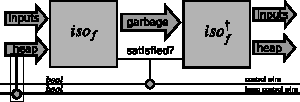
\includegraphics{diagrams/sat2.pdf}
% }
% \end{center}  

% As shown in the circuit, the reversible SAT instance {{iso_f}} takes
% two sets of values and produces two outputs. The incoming values
% labeled \textsf{inputs} are the inputs we need to test for
% satisfiability. The other incoming values labeled \textsf{heap} are
% the additional inputs needed to embed the original SAT instance {{f}}
% into a reversible function. If these \textsf{heap} values are all
% initialized to {{false}}, the output wire \textsf{satisfied?}
% corresponds to the output that {{f}} would have produced on
% \textsf{inputs}. The other outputs labeled \textsf{garbage} are not
% needed for their own sake but they are important because they are used
% as inputs to the adjoint of {{iso_f}} to reproduce the inputs exactly,
% in anticipation of closing the loop with {{trace*}}.

% To summarize, the top half of the circuit is the identity function
% except that we have also managed to produce a boolean wire labeled
% \textsf{satisfied?} that tells us if the inputs satisfy the desired
% constraints. We can take this boolean value and use it to decide
% whether to negate the bottom wire (labeled \textsf{control
%   wire}). Specifically, if the inputs do \emph{not} satisfy {{f}}, the
% control wire is negated. The last wire labeled \textsf{heap control
%   wire} is negated if the heap values do not have the right initial
% values, i.e., are not all {{false}}.

% Let us call the above construction {{sat_f}}. If we now close the loop
% using {{trace*}}, two things should happen:
% \begin{itemize}
% \item configurations in which the \textsf{heap} values are not all
%   {{false}} will be annihilated;
% \item configurations in which the \textsf{inputs} do not satisfy {{f}}
%   will cause the \textsf{satisfied?} wire to be negated and hence will
%   also be annihilated.
% \end{itemize}
% In other words, the only configurations that will survive are the ones in
% which the \textsf{inputs} satisfy {{f}}. We simply need to arrange to
% \emph{clone} these values and produce them as the output of the whole
% circuit. The final construction is therefore:

% \begin{center}
% \scalebox{1.5}{
%   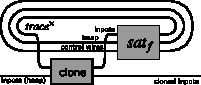
\includegraphics{diagrams/sat3.pdf}
% }
% \end{center}  

% To make the previous discussion concrete, we present a small, but
% complete, example. In our example, the SAT instance {{f}} is tiny: it
% takes two inputs. This function is embedded into a reversible function
% {{iso_f}} of type 
% {{((bool * bool) * bool) <-> ((bool * bool) * bool)}} where the last
% input represents the heap and the first two outputs represent the garbage. 
% The realization of {{sat_f}} given below is parametrized by such 
% a function {{iso_f}}. The inputs to {{sat_f}} are 
% \textsf{heap control}, \textsf{control}, \textsf{heap}, \textsf{input-1}, and 
% \textsf{input-2}. Its operation is simple: if the \textsf{heap} is {{true}}, 
% \textsf{heap control} is negated, and if the last output of {{iso_f}} 
% is {{false}}, \textsf{control} is negated:

% %subcode{opsem} include main
% %! columnStyle = rcl
% % sat_f &:& ((((bool * bool) * bool) * bool) * bool) <-> ((((bool * bool) * bool) * bool) * bool)
% % sat_f &=& ((swap* (*) id) (*) id) (;) 
% % && ((assocl* (*) id) (*) id) (;) 
% % &&   (((cnot (*) id) (*) id) (*) id) (;) 
% % &&   assocr* (;) 
% % &&   (assocr* (*) id) (;) 
% % &&   (swap* (*) id) (;) 
% % &&   assocr* (;) 
% % &&   (id (*) assocl*) (;) 
% % &&   (id (*) isof) (;) 
% % &&   swap* (;) 
% % &&   assocr* (;) 
% % &&   (id (*) (id (*) swap*)) (;) 
% % &&   (id (*) assocl*) (;) 
% % &&   (id (*) ((inot (*) id) (*) id)) (;)
% % &&   (id (*) (cnot (*) id)) (;) 
% % &&   (id (*) ((inot (*) id) (*) id)) (;)
% % &&   (id (*) assocr*) (;) 
% % &&   (id (*) (id (*) swap*)) (;) 
% % &&   assocl* (;)
% % &&   swap* (;)
% % &&   (id (*) Sym isof) (;) 
% % &&   (id (*) assocr*) (;) 
% % &&   assocl* (;) 
% % &&   assocl* 

% Given the construction of {{sat_f}} we can build the full solver as
% follows. The overall input is the cloning heap. The combinator given
% to {{trace*}} takes the cloning heap and the inputs flowing around the
% loop and produces two copies of these inputs. One copy is produced as
% the overall output and another is fed back around the loop. 

% %subcode{opsem} include main
% %! columnStyle = rcl
% % solve_f &:& bool * bool <-> bool * Bool
% % solve_f &=& trace* (
% % && (assocr* (*) id) (;) 
% % && assocr* (;)
% % && (id (*) swap*) (;)
% % && assocl* (;)
% % && (assocr* (*) id) (;)
% % && (clone2 (*) id) (;)
% % && swap* (;)
% % && (swap* (*) id) (;)
% % && ((swap* (*) id) (*) id) (;)
% % && assocl* (;)
% % && assocl* (;)
% % && (sat_f (*) id) (;)
% % && (assocr* (*) id) (;)
% % && (swap* (*) id) (;) 
% % && ((id (*) swap*) (*) id) (;)
% % && (assocl* (*) id) (;)
% % && ((id (*) swap*) (*) id))

% We can test our {{solve_f}} combinator using several SAT
% instances. Here are two possible instances. The first instance is
% satisfied by {{(false,false)}} and the
% second is satisfied by {{(false,true)}} and {{(true,true)}}.

% %subcode{opsem} include main
% %! columnStyle = rcl
% % iso_{f_1} &:& ((bool * bool) * bool) <-> ((bool * bool) * bool)
% % iso_{f_1} &=& (assocr* (;) swap* (;) toffoli (;) swap* (;) assocl*) (;)
% % && (((swap+ (*) id) (*) id) (;) toffoli (;) ((swap+ (*) id) (*) id)) (;) 
% % && (id (*) swap+)
% % 
% % iso_{f_2} &:& ((bool * bool) * bool) <-> ((bool * bool) * bool)
% % iso_{f_2} &=& toffoli

% It can indeed be verified using the semantics that the {{solve_f}}
% combinators instantiated with the SAT instances produce the expected
% results. 

%%%%%%%%%%%%%%%%%%%%%%%%%%%%%%%%%%%%%%%%%%%%%%%%%%%%%%%%%%%%%%%%%%%%%%%%%%%%%
\section{Conclusion}
\label{sec:cat} 

We have introduced the idea of \emph{fractional types} in the context of a
reversible language founded on type isomorphisms and preservation of
information. Values of fractional types represent \emph{negative
  information}, a concept which is difficult to introduce in a conventional
language that allows arbitrary creation and deletion of information but which
is much simpler to deal with when the surrounding language infrastructure
guarantees preservation of information. Fractional types and values can be
used to express a simple and elegant notion of higher-order functions: a
function {{b1 :-* b2}} is a first-class value consisting of negative
information drawn from {{b1}} and positive information drawn from {{b2}}.

The interpretation of our language {{PiTF}} in the category of sets and
relations is adequate in the sense that it produces a language in which every
program is a reversible relation and in which relations are first-class
values. This relational model is however, unsatisfactory, for several
reasons:

\begin{itemize}
\item the type {{1/b}} is interpreted in the same way as {{b}}, which gives no
  insight into the ``true meaning'' of fractionals;
\item the interpretation is inconsistent with the view of types as algebraic
  structures; for example, {{Pi}} with the empty type, is the
  categorification of a semiring but although fractional types in {{PiTF}}
  syntactically ``look like'' rational numbers, there is no such formal
  connection to the rational numbers;
\item finally, we have lost some delicate structure moving from {{Pi}} to
  {{PiTF}} as we can express arbitrary relations between types and not just
  \emph{isomorphisms}.
\end{itemize}

For these reasons, it is interesting to consider other possible semantic
interpretations of fractionals. A natural alternative is to use the
``canonical'' compact closed category, that is finite dimensional vector
spaces and linear maps\cite{Selinger:2011:FDH:1942319.1942398,Hasegawa:2008:FDV:1805839.1805859} over fields of characteristic $0$. Let us fix an arbitrary
field $k$ of characteristic $0$.
Then each type {{b}} in {{PiTF}} is interpreted as a finite dimensional
  vector space $\mathbf{V}_b$ over the field $k$. In particular:
\begin{itemize}
  \item every vector space contains a zero vector which means that the type
    {{0}} (if included in {{PiTF}}) would not be the ``empty'' type.
    Furthermore all combinators would be
    strict as they would have to map the zero vector to itself. 
  \item the type {{1}} is interpreted as a 1-dimensional vector space and hence
    is isomorphic to the underlying field.
  \item the fractional type {{1/b}} is interpreted as the dual vector space
    to the vector space $\mathbf{V}_b$ representing {{b}} consisting of all
    the \emph{linear functionals} on $\mathbf{V}_b$.
  \item one can then validate certain desirable properties: {{1/(1/b)}} is
    isomorphic to {{b}}; and {{eps*_b}} corresponds to a bilinear form which
    maps a dual vector and a vector to a field element.
\end{itemize}

Although this semantics appears to have ``better'' properties than the
relational one, we argue that it is not \emph{the} ``perfect'' semantics. By
including the zero vector, the language has
morphisms that do not correspond to isomorphisms (in particular it allows
partial morphisms by treating the {{0}} element of the zero-dimensional 
vector space as a canonical ``undefined'' value).  It is also difficult to
reconcile the interpretation with the view that the types correspond
to the (positive) rational numbers, something we are actively seeking. What 
would really be a ``perfect'' interpretation is one in which we
can only express {{Pi}}-isomorphisms as first class values and in which the
types are interpreted in a way that is consistent with the rational
numbers. 

Fortunately, there is promising significant work on the groupoid
interpretation of type theory~\cite{Hofmann96thegroupoid} and on the 
categorification of the rational numbers~\cite{math/9802029} that may well give
us the model we desire.  The fundamental idea in both cases is that groupoids
(viewed as sets with explicit isomorphisms as morphisms) naturally have a
\emph{fractional cardinality}.  Types would be interpreted as groupoids, and
terms would be (invertible) groupoid actions.  The remaining challenge is to
identify those groupoid actions which are proper generalizations of
isomorphisms \emph{and} can be represented as groupoids, so as to obtain a
proper interpretation for a higher-order language.  As the category of
groupoids is cartesian closed, this appears eminently feasible.

%%%%%%%%%%%%%%%%%%%%%%%%%%%%%%%%%%%%%%%%%%%%%%%%%%%%%%%%%%%%%%%%%%%%%%%%%%%%%

{\small
\bibliographystyle{splncs03} 
\bibliography{cites}
}
\end{document}

%%%%%%%%%%%%%%%%%%%%%%%%%%%%%%%%%%%%%%%%%%%%%%%%%%%%%%%%%%%%%%%%%%%%%%%%%%%%%
%%%%%%%%%%%%%%%%%%%%%%%%%%%%%%%%%%%%%%%%%%%%%%%%%%%%%%%%%%%%%%%%%%%%%%%%%%%%%

\appendix
\section{Categorical Background}
\label{app:cat} 

We recall that a \emph{symmetric monoidal category} is a category together
with a bifunctor $\otimes$, a distinguished object $I$, and natural
isomorphisms $\alpha_{A,B,C} : (A \otimes B) \otimes C \rightarrow A \otimes
(B \otimes C)$, $\lambda_A : A \rightarrow I \otimes A$, and $\sigma_{A,B} :
A \otimes B \rightarrow B \otimes A$ subject to standard coherence
conditions~\cite{nla.cat-vn1051288}. Following common practice
(e.g.,~\cite{Selinger:2007:DCC:1229185.1229207}), we write $\rho_A =
\sigma_{I,A} \circ \lambda_A : A \rightarrow A \otimes I$.

A \emph{compact closed category} is a symmetric monoidal category where each
object $A$ is assigned a dual object $A^*$, together with a unit map $\eta_A
: I \rightarrow A^* \otimes A$ and a counit map $\epsilon_A : A \otimes A^*
\rightarrow I$, such that:
\[\begin{array}{rcl}
\lambda_A^{-1} \circ (\epsilon_A \otimes A) \circ \alpha_{A,A^*,A}^{-1} \circ (A \otimes \eta_A) \circ \rho_A &=& \mathit{id}_A \\
\rho_{A^*}^{-1} \circ (A^* \otimes \epsilon_A) \circ \alpha_{A^*,A,A^*} \circ (\eta_A \otimes A^*) \circ \lambda_A &=& \mathit{id}_{A^*}
\end{array}\]

A \emph{dagger category} is a category together with an involutive,
identity-on-objects, contravariant functor $\dagger$. Concretely, this means
that to every morphism $F : A \rightarrow B$, one associates a morphism
$f^{\dagger} : B \rightarrow A$, called the \emph{adjoint} of $f$, such that
for all $f : A \rightarrow B$ and $g : B \rightarrow C$, we have:
\[\begin{array}{rcl}
\mathit{id}^\dagger_A &=& \mathit{id}_A \\
(g \circ f)^\dagger &=& f^\dagger \circ g^\dagger \\
(f^\dagger)^\dagger &=& f
\end{array}\]

A \emph{dagger symmetric monoidal category} is a symmetric monoidal category
with a dagger structure such that the contravariant functor $\dagger$
coherently preserves the symmetric monoidal structure. Concretely, this
requirement means that for all $f : A \rightarrow B$ and $g : C \rightarrow
D$, we have:
\[\begin{array}{rcl}
(f \otimes g)^\dagger &=& f^\dagger \otimes g^\dagger \\
\alpha^\dagger_{A,B,C} &=& \alpha^{-1}_{A,B,C} \\
\lambda^\dagger_A &=& \lambda^{-1}_A \\
\sigma^\dagger_{A,B} &=& \sigma^{-1}{A,B}
\end{array}\]

\begin{definition}[Dagger Compact Closed Category]
\label{def:cat}
A \emph{dagger compact closed category} is a dagger symmetric monoidal
category that is also compact closed and such that for all $A$:
\[
\eta_A = \sigma_{A,A^*} \circ \epsilon^\dagger_A
\]
\end{definition}

\todo{biproducts}

\begin{verbatim}
homotopy equivalence???

axioms for field or meadow; actually we probably a semifield

definition of logical reversibility with relations

definition of information preservation in the case of relations; fanout as an
example which we can write

explain in detail the size of 2 * 1/2; it should have exactly one element;
there are two elemens in 2 but the 1/2 identifies them somehow; be precise

we can get the empty relation (eta ; id * swap; eps) what does that mean? 

connection to vector spaces; projectors; inner product. Given dual vectors,
we can have a standalone |0><0| which is a piece of a function or a projector
if viewed by itself; we can also have |v><v'| which produces the scalars YES
or NO. We have an isomorphism between matrices and vectors by viewing 
|0><0|+|1><1| as |00>+|11>

Perhaps if restrict the ``top-level'' to non-fractional types, we can never
observe a function built from from fractionals; we must apply it and in that
case, the system overall behaves like Pi. (no empty relation for example)???
Idea suggested by Zach is to change eps to (1/a) * a * a <-> a

The code implementing the 16 relations... all 16 relations have the same
information content as () ??? So we should treat (1/bool * bool) as opaque
things; we can only extract information from them by applying them.

Include dneg, name (inv cnot) as example of programs which when fed
non-fractional values produce fractional values

Also include recipT which shows that 1/ distributes over products and tens
which shows that we can manipulate fractional types in interesting ways

Using relational semantics is good because it's clear; but it's also bad
unless we spend time to explain the operational model

Explain 'name' in detail; it IS a faithful representation of the input
relation as a value; we don't get to see the full relation though; we
interact with it by giving it inputs and observing the related ouptut come
out. If we make two copies and use each in a different context (applying each
to a different value, we can ``see'' that it's really a full relation and not
just one branch.) 

total functions have size 1; partial functions have fractional sizes!!!

denotation of type in Pi is a set; in Pi/ we get a set with an equivalence
relation (Id by default) but fractionals introduce first-class equivalence
relations that can be used to restrict the sets.

---

Having re-read Baez-Dolan, I now feel better.

On 13-02-08 08:53 AM, Amr Sabry wrote:
> I think all the observations in this email are due to the fact that we
> haven't formalized the size of fractionals using homotopy equivalence. I
> started doing this but abandoned it for now but the bottom line is that
> the size of b * 1/b is 1.

Again, agree - more deeply so now.  In more detail, my current thinking:
- v \in b has size 1.  So |b| counts how many elements it has, whenever 
b is a type of Pi.  The sum and product rules apply.
- for b * 1/b to have size 1, then 1/b must have size 1/|b| (assuming 
these are independent types, which we have been assuming all along)

Attempt #1
- there are |b| elements in 1/b, and if size is additive, ( 1/|b| = 
sum_{1/v \in 1/b} |1/v| ) should hold; since |1/v| should be constant, 
this sum is |b|*c, so c = 1/|b|^2.  Weird.

Let us look at a single 'function' in bool -o bool, namely the identity 
function.  It should be 'the same' as { (1/true, true), (1/false, false) 
}.  The cardinality of that set is (1/(2^2)*1 + 1/(2^2)*1) = 1/4 + 1/4 = 
1/2.   From weird to probably-wrong.

Attempt #2
- the elements of 1/b are not distinguishable from each other (i.e. they 
are all isomorphic).  So each element 1/v has b automorphisms, so |1/b| 
= sum_{aut classes of 1/v \in 1/b} 1/|aut 1/v| = sum_{singleton} 1/|b| = 
1/|b|.  [as per p.14 of Baez-Dolan]

The size of the set { (1/true, true), (1/false, false) } is now 1/2*1 + 
1/2*1 = 1.  So this 'set' indeed represents a single "concept".

Note that in attempt #2, we get a new phenomenon.  Consider the 
(partial) relation {(1/true, false)}, also of type bool -o bool.  It has 
size 1/2 !  So, if I have not erred somewhere, only total functions have 
size 1.  Which, I must admit, I rather like.  It's not that partial 
functions are outlawed, they just don't pull as much weight [pun intended].

So 1/b is very much like a collection of |b| constraints, all of which 
are "the same" (externally).  While they may have internal structure, it 
is not visible to any of our combinators, so up to iso, there is only a 
single element of 1/b, of size 1/|b|.

Yet another way to look at it: let's assume we are looking at FinSet_0, 
where in fact our universe U has finitely (say N) things in it.  Then 
the singleton set 1 is actually the isomorphism class of {u_1, ..., 
u_N}.  There are N of them, but they have N automorphisms in a single 
orbit, so the quotient has size 1 (i.e. |S| = N but |G| = N too, so |S 
// G| = 1 ).

So an element of 1/b is closer to an action of b on b; we call it a 
constraint, or a pattern-match.  I think thinking of it as 'actions' is 
definitely the right way to go, as we will be able to have different 
kinds of actions on a type b that just those that come from the elements.

> I don't know how much of a priority this is but if it is we should try
> to work it out in detail. The good and bad news is that we will have a
> model much richer and much more complicated than relations. My thought
> when writing sec. 3 was that we would use the simple but slightly
> inadequate model of relations (which for one thing confuses v and 1/v)
> and simply mention that the right abstraction is that of 'biproduct
> dagger compact closed categories' which presumably would include the
> richer model.

I am as convinced that the right model is 'biproduct dagger compact 
closed categories' as I am that the right model for the type level is 
'categorified field'.

\end{verbatim}

\begin{comment}
Each type in {{PiTF}} is interpreted as a \emph{groupoid}. A groupoid can be
equivalently viewed as an oriented graph, a generalization of a group, or a
special category. We present the categorical view below.

A groupoid is defined by:
\begin{itemize}
\item a set of objects $x,y,\ldots$;
\item for each pair of objects, a (possibly empty) set $G(x,y)$ of morphisms
  $x \rightarrow y$; 
\item for each object $x$, there exists an identity morphism {{id_x in G(x,x)}};
\item for each triple of objects $x,y,z$, we have a function 
{{comp_{x,y,z} : G(x,y) * G(y,z) -> G(x,z)}}
\item there exists a function {{inv_{x,y} : G(x,y) -> G(y,x)}}
\end{itemize}
such that for all {{f : x -> y}}, {{g : y -> z}}, and {{h : z -> w}}, we have:
%subcode{bnf} include main
% comp_{x,x,y}(id_x,f) &=& f \\
% comp_{x,y,y}(f,id_y) &=& f \\
% comp_{x,y,z}(f, comp_{y,z,w}(g,h)) &=& comp_{x,z,w}(comp_{x,y,z}(f,g),h) \\
% comp_{y,x,y}(inv_{x,y}(f),f) &=& id_y \\
% comp_{x,y,x}(f,inv_{x,y}(f)) &=& id_x

We now proceed to explain how each {{PiTF}} type denotes a groupoid. First,
each {{Pi}} type denotes a set as follows.

\begin{definition}[Denotation of {{Pi}} Value Types {{ [[ b ]] }}]
\label{chx:def:denot}
Each {{Pi}}type denotes a finite set of values as follows:
%subcode{opsem} include main
%! <- = \leftarrow
%! union = \cup
% [[1]] '= {[ () ]}
% [[b1 + b2]] '= {[ left v ~|~ v <- [[b1]] ]} union {[ right v ~|~ v <- [[b2]] ]}
% [[b1 * b2]] '= {[ (v1, v2) ~|~ v1 <- [[b1]], v2 <- [[b2]] ]}
\end{definition}

For each of the types {{b}} above, the corresponding groupoid consists of the
set {{ [[b]] }} of elements with only the trivial identity morphisms. The
interesting groupoid is the one associated with {{1/b}}. It is defined as
follows. 

Fractional types and values add considerable expressiveness to our
language. 
\end{comment}

If it were not for the cases of {{eta*}} and {{eps*}}, each combinator 
{{c : b1 <-> b2}} would define a total one-to-one function between the sets 
{{ [[ b1 ]] }} and {{ [[ b2 ]] }}. 
This is indeed the situation for the language {{Pi}} 
defined in the previous section. In the presence of fractionals, this simple 
interpretation of combinators as one-to-one functions is not sufficient%
\footnote{The interpretation of combinators as one-to-one functions is also 
not valid in the presence of recursive 
types~\cite{rc2011,James:2012:IE:2103656.2103667}.}.
The intuitive reason, is that the fission point combinator 
{{eta*_b : 1 <-> 1/b * b}} must be
able to map the element {{() : 1}} to any pair of the form {{(1/v,v)}} with
{{v:b}}. Similarly, the combinator {{eps*_b : 1/b * b <-> 1}} must be able to
accept pairs {{(1/v1,v2)}} in which the negative information {{1/v1}} does
not match the positive information {{v2}}. On such pairs, {{eps*_b}} is
undefined, i.e., it does not produce {{():1}}. 

discuss two generalizations of the semantics

vector spaces (more refined because it doesn't collapse 1/b to b; also each
vector space must have a zero vector; so we have an explicit notion of
``error'' which we can use and track at run time. Adding this error
eliminates at RUN TIME relations which are not isomorphisms I think. 

a potentially better and more semantics is based on groupoids; mention that
we can have sets (with structure) who cardinality is fractionals and that this
would formalize nicely the negative information


\newunicodechar{≟}{$\mathbin{\stackrel{?}{=}}$}
\newunicodechar{𝕌}{$\mathbb{U}$}
\newunicodechar{𝔹}{$\mathbb{B}$}
\newunicodechar{𝔽}{$\mathbb{F}$}
\newunicodechar{𝕋}{$\mathbb{T}$}
\newunicodechar{𝟘}{$\mathbb{0}$}
\newunicodechar{𝟙}{$\mathbb{1}$}
\newunicodechar{𝟚}{$\mathbb{2}$}
\newunicodechar{⋆}{${}_*$}
\newunicodechar{○}{$\gcv$}
\newunicodechar{ᵤ}{${}_u$}
\newunicodechar{⊚}{$\fatsemi$}
\newunicodechar{⟷}{$\leftrightarrow$}
\newunicodechar{⟶}{$\longrightarrow$}
\newunicodechar{⟪}{$\ll$}
\newunicodechar{⟫}{$\gg$}
\newunicodechar{⊎}{$\uplus$}
\newunicodechar{ₗ}{$_l$}
\newunicodechar{ᵣ}{$_r$}

\newcommand{\alt}{~|~}
\newcommand{\net}{t_\bullet}
\newcommand{\gcv}{\circlearrowright}
\newcommand{\opr}[1]{|#1\rangle\langle#1|}
\newcommand{\inlv}[1]{\ensuremath{\mathit{inl}(v)}}
\newcommand{\inrv}[1]{\ensuremath{\mathit{inr}(v)}}
\newcommand{\ket}[1]{|#1\rangle}
\newcommand{\oneover}[1]{1/#1}
\newcommand{\pointed}[2]{[#1 \bullet #2]}
\newcommand{\nboxtimes}[2]{\,\,~{^{#1}\boxtimes^{#2}}~\,\,}
\newcommand{\mm}{\texttt{\textminus}}
\newcommand{\pp}{\texttt{+}}
\newcommand{\inl}[1]{\textsf{inl}~#1}
\newcommand{\inr}[1]{\textsf{inr}~#1}
\newcommand{\idv}[3]{#2 \xrightarrow{#1} #3}
\newcommand{\cp}[3]{#1\stackrel{#2}{\bullet}#3}
\newcommand{\idt}[3]{#2 \equiv_{#1} #3}
\newcommand{\idrt}[3]{#3 \equiv_{#1} #2}
\newcommand{\refl}[1]{\textsf{refl}~#1}
\newcommand{\lid}{\textsf{lid}}
\newcommand{\rid}{\textsf{rid}}
\newcommand{\linv}{l!}
\newcommand{\rinv}{r!}
\newcommand{\invinv}{!!}
\newcommand{\assoc}{\circ}
\newcommand{\identlp}{\mathit{unite}_+\mathit{l}}
\newcommand{\identrp}{\mathit{uniti}_+\mathit{l}}
\newcommand{\identlsp}{\mathit{unite}_+\mathit{r}}
\newcommand{\identrsp}{\mathit{uniti}_+\mathit{r}}
\newcommand{\swapp}{\mathit{swap}_+}
\newcommand{\assoclp}{\mathit{assocl}_+}
\newcommand{\assocrp}{\mathit{assocr}_+}
\newcommand{\identlt}{\mathit{unite}_*\mathit{l}}
\newcommand{\identrt}{\mathit{uniti}_*\mathit{l}}
\newcommand{\identlst}{\mathit{unite}_*\mathit{r}}
\newcommand{\identrst}{\mathit{uniti}_*\mathit{r}}
\newcommand{\swapt}{\mathit{swap}_*}
\newcommand{\assoclt}{\mathit{assocl}_*}
\newcommand{\assocrt}{\mathit{assocr}_*}
\newcommand{\absorbr}{\mathit{absorbr}}
\newcommand{\absorbl}{\mathit{absorbl}}
\newcommand{\factorzr}{\mathit{factorzr}}
\newcommand{\factorzl}{\mathit{factorzl}}
\newcommand{\dist}{\mathit{dist}}
\newcommand{\factor}{\mathit{factor}}
\newcommand{\distl}{\mathit{distl}}
\newcommand{\factorl}{\mathit{factorl}}
\newcommand{\distz}{\mathit{absorbr}}
\newcommand{\iso}{\leftrightarrow}
\newcommand{\proves}{\vdash}
\newcommand{\idc}{\mathit{id}\!\!\leftrightarrow}
\newcommand{\Rule}[4]{
\makebox{{\rm #1}
$\displaystyle
\frac{\begin{array}{l}#2 \\\end{array}}
{\begin{array}{l}#3      \\\end{array}}$
 #4}}
\newcommand{\jdg}[3]{#2 \proves_{#1} #3}
\renewcommand{\AgdaCodeStyle}{\small}
% 12 pages

%%%%%%%%%%%%%%%%%%%%%%%%%%%%%%%%%%%%%%%%%%%%%%%%%%%%%%%%%%%%%%%%%%%%%%%%%%%
\begin{document}

\title{Fractional Types}
\subtitle{Expressive and Safe Space Management for Ancilla Bits}
\author{Chao-Hong Chen}
\affiliation{
  \institution{Indiana University}
}

\author{Vikraman Choudhury}
\affiliation{
  \institution{Indiana University}
}

\author{Jacques Carette}
\affiliation{
  \institution{McMaster University}
}

\author{Amr Sabry}
\affiliation{
  \institution{Indiana University}
}

\begin{abstract}
  In reversible and quantum computing, the management of space is
  subject to two broad classes of constraints. First, as is the case
  for general-purpose computation, every allocation must be paired
  with a matching de-allocation. Second, space can only be safely
  de-allocated if its contents are restored to their initial value
  from allocation time. Generally speaking, the state of the art
  provides limited partial solutions that address the first
  constraint by imposing a stack discipline and by leaving the second
  constraint to programmer's assertions.

  We propose a novel approach based on the idea of \emph{fractional
    types}. As a simple intuitive example, allocation of a new boolean
  value initialized to \textsf{false} also creates a value
  $\oneover{\textsf{false}}$ that can be thought of as a garbage
  collection (gc) process specialized to reclaim, and only reclaim,
  storage containing the value $\textsf{false}$. This gc process is a
  first-class entity that can sliced and diced by combining it with
  other gc processes and decomposing it in smaller
  processes.

  Technically, we formalize this idea in the context of a reversible
  language founded on type isomorphisms, prove its fundamental
  correctness properties, and illustrate its expressiveness using a
  wide variety of examples. The development is backed by a
  fully-formalized Agda implementation.
\end{abstract}

\maketitle

\input{latex/PiFracDynDefCode.tex}
\input{latex/PiFracDynCode.tex}
\input{latex/BooleanCircuitsCode.tex}
\input{latex/PiPointedFracCode.tex}
\input{latex/ExtractionCode.tex}
\input{latex/PiMemSemCode.tex}
\input{latex/PiFracMemSemCode.tex}
\input{latex/J.tex}

%%%%%%%%%%%%%%%%%%%%%%%%%%%%%%%%%%%%%%%%%%%%%%%%%%%%%%%%%%%%%%%%%%%%%%%%%%%
\section{Introduction}

If quantum field theory is correct (as it so far seems to be) then
information, during any physical process, is neither created nor
destroyed. Landauer~\cite{Landauer:1961,Landauer,bennett1985fundamental},
Bennett~\cite{bennett2010notes,bennett2003notes,Bennett:1973:LRC},
Fredkin~\cite{fredkin1982conservative} and others made compelling
arguments that this physical principle induces a corresponding
computational principle of ``conservation of information.'' This
principle is indeed one of the defining characteristics of quantum
computing and its classical restriction known as reversible computing.

\paragraph*{Quantum and Reversible Computing Based on Type
  Isomorphisms.} The Toffoli gate is known to be universal for
classical reversible circuits~\cite{Toffoli:1980}. Adding just one
gate (the Hadamard gate) produces a universal set of primitives for
quantum circuits~\cite{hadtoffuniv}. The ``only'' difference between
the two circuit models is that quantum circuits can process
superpositions of values (waves) in one step whereas classical
circuits lack this form of parallelism. Most importantly, structurally
the two circuits models are identical and one can derive properties
valid for both families by focusing on the simpler classical model. In
fact, classical reversible computations are often used as
``subroutines'' of quantum computations. Indeed classical reversible
circuits can be applied to either classical inputs or to quantum
inputs. 

Instead of using the rather low-level circuit model of computation,
one can leverage the full force of type theory and category theory by
expressing reversible classical computations as \emph{isomorphisms
  over finite types}~\cite{Fiore:2004,James:2012:IE:2103656.2103667}
or \emph{equivalences over
  groupoids}~\cite{DBLP:conf/esop/CaretteS16}. This perspective is
similarly universal for reversible computation (and can be extended to
quantum computation~\cite{10.1007/978-3-319-89366-2_19}) but with the
advantage of exposing a rich mathematical structure in reversible
computations that we will exploit to solve the ``ancilla problem''
explained next.

\paragraph*{Temporary Storage using Ancilla Bits.} The universality of
the Toffoli gate for classical reversible computing and of the
universality of the Toffoli-Hadamard gates for quantum computing should
not distract from efficiency and safety concerns. The theorems proving
universality (i) assume that temporary storage (often called
\emph{ancilla bits}) may be used~\cite{Toffoli:1980}, and (ii) that
this temporary storage is returned to its initial state before
de-allocation. Indeed if no temporary storage is allowed, the Toffoli
gate is not
universal~\cite{DBLP:conf/innovations/AaronsonGS17,DBLP:journals/corr/Xu15e}
and as would be expected the more temporary storage is allowed, the
more efficient certain computations could become.

More fundamentally, the condition requiring that the temporary storage
is only de-allocated when returned to its initial condition is a
safety condition. Violating this condition destroys the symmetry
between input and output making the circuits not reversible and, in
the quantum model, causes decoherence that may destroy the quantum
state. As reviewed in Sec.~\ref{sec:examples}, ancilla bits have a
number of critical applications and yet are poorly supported in
current reversible and quantum programming languages making them a
common source of bugs.

\paragraph*{Conservation of Information and Negative Entropy.}  
According to the conventional theory of
communication~\cite{Shannon1948}, a type with $N$ values is viewed as
an abstract system that has $N$ distinguishable states where the
amount of information contained in each state is $\log{N}$. This
entropy is a measure of information which materializes itself in
memory or bandwidth requirements when storing or transmitting elements
of this type. Thus a type with 8 elements needs 3 bits of memory for
storage or 3 bits of bandwidth for communication. The logarithmic map
implies that information contained in a composite state is the sum of
the information contained in its constituents. For example, the type
$A \times B$ where $A$ has two elements and $B$ has three elements can
be thought of a composite system consisting of two independent
unrelated subsystems.  Each state of the composite system therefore
contains $\log{(2*3)} = \log{2} + \log{3}$ bits which is the sum of
the information contained in each subsystem. If we could imagine a
\emph{fractional type} $\frac{1}{A}$, this type would introduce
negative entropy. For example, a type with ``cardinality''
$\frac{1}{8}$ has entropy $\log{\frac{1}{8}} = -3$. It is natural to
interpret this negative entropy just like we interpret ``negative
money,'' as a resource (space or bandwidth) to be repaid (reclaimed)
by some other part of the system. Indeed, we will introduce such
fractional types and use them to represent ``garbage collection
processes'' that reclaim temporary storage. Just like in the case of
``negative money'' it is critical that these fractional types be
linearly used, i.e., they cannot be duplicated or erased: this
property is however automatically enforced in a reversible
computational model.

\paragraph*{Outline.} The paper solves the ancilla problem in
reversible and quantum computation using a novel concept:
\emph{fractional types}. In the next section, we introduce the problem
of ancilla, motivate its importance, and explain the limitations of
current solutions. In Sec.~\ref{sec:pi}, we review existing work by
James et al.~\cite{rc2011,rc2012,James:2012:IE:2103656.2103667} that
introduces a reversible programming language built using isomorphism
of types. Although it is conceivable that the concept of fractional
types would apply to general-purpose languages (after some
adaptation), its natural technical definition exploits symmetries
present in categorical model of type isomorphisms. We present such a
definition in Sec.~\ref{sec:dyn} which captures and illustrates the
main novelties of fractional types and their runtime representations
as first-class gc processes. This presentation partially solves a more
general and more expressive instance of the ancilla problem as
illustrated with examples. To make the arguments regarding memory
management explicit, Sec.~\ref{sec:space} presents an abstract machine
with a heap component that grows and shrinks as ancillae are allocated
and de-allocated via fractional gc processes. In Sec.~\ref{sec:dep} we
lift ``plain'' programs manipulating ancillae to the type system in
order to exploit the power of dependent types to guarantee, for the
first time, the condition necessary for safe de-allocation of
ancillae. Technically this solution requires the introduction of
pointed types on top of which are defined both a monad and co-monad of
singleton types. The tracking of ancillae value is done within the
type system via the singleton types. A number of examples exploiting
the singleton-based type system are present to demonstrate the full
expressiveness of fractional types. We furthermore demonstrate that,
from the proofs of type safety, plain (but guaranteed to be safe)
programs can be extracted and executing without errors or runtime
checks in the conventional type system. The last section concludes
with a discussion of related work and a summary of our results.

%%%%%%%%%%%%%%%%%%%%%%%%%%%%%%%%%%%%%%%%%%%%%%%%%%%%%%%%%%%%%%%%%%%%%%%%%%%
\section{Ancilla Bits}
\label{sec:examples}
 
Restricting a reversible (classical or quantum) circuit to use no
ancillae is like restricting a Turing machine to use no memory other
than the $n$ bits used to represent the
input~\cite{DBLP:conf/innovations/AaronsonGS17}. As such a restriction
disallows countless computations for trivial reasons, reversible and
quantum models of computation have, since their inception, included
management for scratch storage in the form of ancilla
bits~\cite{Toffoli:1980} with the fundamental restriction that such
bits must be returned to their initial states before being safely
reused or de-allocated.

%%%
\subsection{Applications}
 
Beyond computability and efficiency reasons, ancillae have found a
wide range of interesting applications. 

\paragraph*{Quantum blackboxes and Phase Kickback Trick.} Consider a
small database with four elements $a$, $b$, $c$, and $d$. We are given
a function $f$ that maps every element to $0$ except for one element
of interest, e.g., $f(a)=1$ and $f(b)=f(c)=f(d)=0$. In the worst case,
finding the element of interest might require applying $f$ to every
element of the database. In the quantum world we can find the element
much more efficiently using Grover's
algorithm~\cite{Grover:1996:FQM:237814.237866}. We start by building
an equally weighted superposition of the elements:
$\frac{1}{2}\ket{a}+\frac{1}{2}\ket{b}+\frac{1}{2}\ket{c}+\frac{1}{2}\ket{d}$
and operate concurrently of the superposition as follows:

\[\begin{array}{l}
                    \frac{1}{2}\ket{a}+\frac{1}{2}\ket{b}+\frac{1}{2}\ket{c}+\frac{1}{2}\ket{d}\\
\\
\Rightarrow  \textrm{phase kickback} \\
\\
-\frac{1}{2}\ket{a}+\frac{1}{2}\ket{b}+\frac{1}{2}\ket{c}+\frac{1}{2}\ket{d}\\
\\
\Rightarrow  \textrm{diffusion} \\
\\
 (\frac{1}{2}-(-\frac{1}{2}))\ket{a}+(\frac{1}{2}-\frac{1}{2})\ket{b}+(\frac{1}{2}-\frac{1}{2})\ket{c}+(\frac{1}{2}-\frac{1}{2})\ket{d})\\
\\
\Rightarrow  \textrm{simplification} \\
\\
\ket{a}
\end{array}\]

The question, which arises repeatedly in quantum computation, is how
to implement operations such as phase kickback. Essentially we want to
concurrently perform the following action on every element of the
superposition:
\[\begin{array}{l}
  \textbf{if}~\textit{current-element}=\ket{a} \\
  \textbf{then}~\textit{negate} \\
  \textbf{else}~\textit{identity}
\end{array}\]
In the quantum world, na\"\i vely attempting to test whether the
current element is equal to $\ket{a}$ by performing a measurement would
destroy the quantum superposition defeating the entire algorithm.

Here is where ancilla qubits come to the rescue. In the words of
Matuschak and Nielsen~\cite{howgrover}, the idea is the following:
\begin{quote}
  There's a rough heuristic worth noting here, which is that you can
  often convert \verb|if-then| style of thinking into quantum
  circuits. You introduce an ancilla qubit to store the outcome of
  evaluating the \verb|if| condition. And then depending on the state
  of the ancilla, you perform the appropriate state
  manipulation. Finally, when possible you reverse the initial
  computation, resetting the ancilla to its original state so you can
  subsequently ignore it.
\end{quote}

\paragraph*{Quantum Error Correction.} The main requirement for
quantum error correction is the ability to replicate the state of a
qubit onto a number of qubits~\cite[Ch.~3]{NAP25196}. This is however
impossible to do directly by the no-cloning theorem~\cite{XXX}. Again ancilla
qubits come to the rescue: because ancilla qubits start in a known
initial state, it is possible to create a simple circuit that makes
their output state match a protected qubit without knowing or
disturbing the protected qubit. Chong et al.~\cite{sigarchblog}
illustrate the idea with a simple example:
\begin{quote}
consider a 3-qubit quantum majority code in which a logical ``0'' is
encoded as ``000'' and a logical ``1'' is encoded as ``111.''  Just as with
a classical majority code, a single bit-flip error can be corrected by
restoring to the majority value.  Unlike a classical code, however, we
can not directly measure the qubits else their quantum state will be
destroyed.  Instead, we measure syndromes from each possible pair of
qubits by interacting them with an ancilla, then measure each ancilla.
Although the errors to the qubits are actually continuous, the effect
of measuring the ancilla is to discretize the errors, as well as
inform us whether an error occurred so that it can be corrected.  
\end{quote}

\paragraph*{Deferring Quantum Measurements.} The evolution of a
quantum system is deterministic. Measurement add significant
complications, collapsing the quantum state, and producing
probabilistic results. However, using ancilla qubits it is possible to
avoid doing any intermediate measurements in a quantum
circuit~\cite{dewolf}. 

%%%
\subsection{Ancillae Bugs in Benchmarks.}
Despite its fundamental importance, the management of ancillae is
poorly supported in current languages, simulators, and toolkits as
demonstrated in a recent analysis of bugs in quantum
benchmarks~\cite{DBLP:conf/oopsla/HuangM18}. The analysis reveals that
lack of language support in the management of ancillae leads to
several problems. For example: 
\begin{quote}
  \textbf{Bug type 6: Incorrect composition of operations using mirroring}
  Section~4.5 discussed how bugs in deallocating ancillary qubits can
  happen due to bad parameters. Here we see how bugs in deallocating
  ancillary qubits can happen due to incorrect composition of
  operations following a mirroring pattern. For example, in Table~7,
  the operations in rows 2 and 3 are respectively mirrored and undone
  in rows~6 and~5. These lines of code need careful reversal of every
  loop and every operation.
\end{quote}

%%%%%%%%%%%%%%%%%%%%%%%%%%%%%%%%%%%%%%%%%%%%%%%%%%%%%%%%%%%%%%%%%%%%%%%%%%%
\begin{figure*}[t]
\begin{multicols}{2}
\[\begin{array}{rrcll}
\idc :& \tau & \iso & \tau &: \idc \\
\\
\identlp :&  0 + \tau & \iso & \tau &: \identrp \\
\swapp :&  \tau_1 + \tau_2 & \iso & \tau_2 + \tau_1 &: \swapp \\
\assoclp :&  \tau_1 + (\tau_2 + \tau_3) & \iso & (\tau_1 + \tau_2) + \tau_3 &: \assocrp \\
\\
\identlt :&  1 * \tau & \iso & \tau &: \identrt \\
\swapt :&  \tau_1 * \tau_2 & \iso & \tau_2 * \tau_1 &: \swapt \\
\assoclt :&  \tau_1 * (\tau_2 * \tau_3) & \iso & (\tau_1 * \tau_2) * \tau_3 &: \assocrt \\
\\
\distz :&~ 0 * \tau & \iso & 0 ~ &: \factorzl \\
\dist :&~ (\tau_1 + \tau_2) * \tau_3 & \iso & (\tau_1 * \tau_3) + (\tau_2 * \tau_3)~ &: \factor
\end{array}\]
\vspace{2cm}
\begin{center}
\Rule{}
{\jdg{}{}{c_1 : \tau_1 \iso \tau_2} \quad \vdash c_2 : \tau_2 \iso \tau_3}
{\jdg{}{}{c_1 \fatsemi c_2 : \tau_1 \iso \tau_3}}
{}

\vspace{1cm}

\Rule{}
{\jdg{}{}{c_1 : \tau_1 \iso \tau_2} \quad \vdash c_2 : \tau_3 \iso \tau_4}
{\jdg{}{}{c_1 \oplus c_2 : \tau_1 + \tau_3 \iso \tau_2 + \tau_4}}
{}

\vspace{1cm}

\Rule{}
{\jdg{}{}{c_1 : \tau_1 \iso \tau_2} \quad \vdash c_2 : \tau_3 \iso \tau_4}
{\jdg{}{}{c_1 \otimes c_2 : \tau_1 * \tau_3 \iso \tau_2 * \tau_4}}
{}
\end{center}
\end{multicols}
\caption{$\Pi$-terms and combinators.}
\label{pi-terms}
\end{figure*}

\section{Preliminaries: $\Pi$}
\label{sec:pi}

The step from reversible classical circuits to quantum circuits
requires the addition of just one gate that creates
superpositions. Similarly the step from a reversible classical
programming language to a quantum one requires just the management of
superpositions, for example starting from the classical reversible
language Theseus~\cite{james2014theseus}, a small extension produces a quantum
language with quantum control~\cite{10.1007/978-3-319-89366-2_19}. The
language Theseus~\cite{james2014theseus} mentioned above is a language that uses
convenient syntactic extensions over an more basic language $\Pi$ of
combinators witnessing isomorphisms over finite types~\cite{XXX}. The
combinator-based language has the advantage of being more amenable to
formal analysis for at least two reasons: (i) it is conceptually
simple and small, and (ii) it has direct and evident connections to
type theory and category theory. Indeed our solution for managing
ancillae is inspired by the construction of \emph{compact closed
  categories}~\cite{XXX}. These categories extend the monoidal
categories~\cite{XXX} which are used to model many resource-aware
programming languages~\cite{XXX} (including $\Pi$) with a new type
constructor that creates duals or inverses to existing types. This
dual will be our fractional type.

%%%%%
\subsection{Core $\Pi$}
\label{sub:core}

The syntax of the language consists of several categories:
\[\begin{array}{lrcl}
\textit{Value types} & t &::=& 0 \alt 1 \alt t+t \alt t*t \\
\textit{Values}      & v &::=& \star \alt \inlv{v} \alt \inrv{v} \alt (v,v) \\
\textit{Level-1 types} &&& t \leftrightarrow t \\
\textit{Level-1 programs} & c &::=& (\textrm{See Fig.~\ref{pi-terms}})\\
\textit{Level-2 types} &&& c \Leftrightarrow c \\
\textit{Level-2 programs} & \alpha &::=& (\textrm{Omitted})
\end{array}\]

Focusing on finite types, the building blocks of type theory are: the
empty type ($0$), the unit type ($1$), the sum type ($+$), and the
product ($\times$) type. One may view each type $A$ as a collection of
physical wires that can transmit $\|A\|$ distinct values where $\|A\|$
is the size of a type, computed as: $\| 0 \| = 0$; $\| 1 \| = 1$;
$\| A + B \| = \| A \| + \| B \|$; and
$\| A \times B \| = \| A \| * \| B \|$. Thus the type
$\mathbb{B} = 1 + 1$ corresponds to a wire that can transmit two
values, i.e., bits, and the type
$\mathbb{B} \times \mathbb{B} \times \mathbb{B}$ corresponds to a
collection of wires that can transmit three bits. From that
perspective, a type isomorphism between types $A$ and $B$ (such that
$\|A\|=\|B\|=n$) models a \emph{reversible} combinational circuit that
\emph{permutes} the $n$ different values. These type isomorphisms are
collected in Fig.~\ref{pi-terms}. It is known that these type
isomorphisms are sound and complete for all permutations on finite
types~\cite{Fiore:2004,fiore-remarks} and hence that they are
\emph{complete} for expressing combinational
circuits~\cite{fredkin1982conservative,James:2012:IE:2103656.2103667,Toffoli:1980}. Algebraically,
these types and combinators form a \emph{commutative semiring} (up to
type isomorphism). Logically they form a superstructural logic
capturing space-time tradeoffs~\cite{superstructural}. Categorically,
they form a \emph{bimonoidal category}~\cite{laplaza72}. 

So far, the types encode conventional data structures, i.e, sets of
values and structured trees of values and the isomorphisms act on such
conventional data structures. Universal computation models however
fundamentally rely on the fact that \emph{programs are (or can be
  encoded as) data}, e.g., a Turing machine can be encoded as a string
that another Turing machine (or even the same machine) can
manipulate. In our setting, we ask whether the type isomorphisms in
Fig.~\ref{pi-terms} can themselves be subject to (higher-level)
reversible deformations? The answer is
yes~\cite{Miller:2003:TBA:775832.775915,DBLP:conf/esop/CaretteS16,DBLP:journals/corr/CockettCS17}. We
only give one example below. (We will require a new level-2 program to
witness coherence of fractional types in Sec.~\ref{sec:dep}.)

\begin{center}
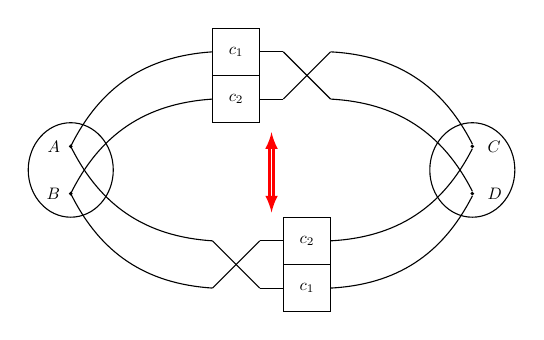
\begin{tikzpicture}[scale=0.6,every node/.style={scale=0.6}]
  \draw[>=latex,<->,double,red,thick] (2.25,-1.2) -- (2.25,-2.9) ;
  \draw (-2,-2) ellipse (0.9cm and 1cm);
  \draw[fill] (-2,-1.5) circle [radius=0.025];
  \node[left] at (-2.1,-1.5) {$A$};
  \draw[fill] (-2,-2.5) circle [radius=0.025];
  \node[left] at (-2.1,-2.5) {$B$};

  \draw (6.5,-2) ellipse (0.9cm and 1cm);
  \draw[fill] (6.5,-1.5) circle [radius=0.025];
  \node[right] at (6.7,-1.5) {$C$};
  \draw[fill] (6.5,-2.5) circle [radius=0.025];
  \node[right] at (6.7,-2.5) {$D$};

  \draw[-] (-2,-1.5) to[bend left] (1,0.5) ;
  \draw[-] (-2,-2.5) to[bend left] (1,-0.5) ;
  \draw[-] (3.5,0.5) to[bend left] (6.5,-1.45) ;
  \draw[-] (3.5,-0.5) to[bend left] (6.5,-2.45) ;

  \draw[-] (-2,-1.5) to[bend right] (1,-3.5) ;
  \draw[-] (-2,-2.5) to[bend right] (1,-4.5) ;
  \draw[-] (3.5,-3.5) to[bend right] (6.5,-1.55) ;
  \draw[-] (3.5,-4.5) to[bend right] (6.5,-2.55) ;

  \draw     (2.5,-3)  -- (3.5,-3) -- (3.5,-4) -- (2.5,-4) -- cycle ;
  \draw     (2.5,-4)  -- (3.5,-4) -- (3.5,-5) -- (2.5,-5) -- cycle ;

  \draw     (1,1)  -- (2,1) -- (2,0) -- (1,0) -- cycle ;
  \draw     (1,0)  -- (2,0) -- (2,-1) -- (1,-1) -- cycle ;

  \node at (3,-3.5) {$c_2$};
  \node at (3,-4.5) {$c_1$};

  \node at (1.5,0.5) {$c_1$};
  \node at (1.5,-0.5) {$c_2$};

  \draw     (2,0.5)  -- (2.5,0.5)  ;
  \draw     (2,-0.5) -- (2.5,-0.5) ;

  \draw     (2.5,0.5)  -- (3.5,-0.5)  ;
  \draw     (2.5,-0.5) -- (3.5,0.5) ;

  \draw     (1,-3.5)  -- (2,-4.5)    ;
  \draw     (1,-4.5) -- (2,-3.5)   ;

  \draw     (2,-3.5)  -- (2.5,-3.5)    ;
  \draw     (2,-4.5) -- (2.5,-4.5)   ;

\end{tikzpicture}
\end{center}

\noindent The top path is the $\Pi$ program
$(c_1~\oplus~c_2)~\fatsemi~\swapp$ which acts on the type $A$ by $c_1$,
acts on the type $B$ by $c_2$, and deforms the resulting space by a
twist that exchanges the two injections into the sum type. The bottom
path performs the twist first and then acts on the type $A$ by $c_1$
and on the type $B$ by $c_2$ as before. If one could imagine the paths
as physical wires and the actions $c_1$ and $c_2$ as permutations on
these wires then, holding the points $A$, $B$, $C$, and $D$ fixed, it
is possible to rotate the top part of the diagram to become identical
to the bottom one. That rotation can be undone (reversed), which takes
the bottom part of the diagram into the top part.  In other words,
there exists a continuous deformation of the program
$(c_1~\oplus~c_2)~\fatsemi~\swapp$ to the program
$\swapp \fatsemi (c_2~\oplus~c_1)$. We can also show that this means
that, as permutations, $(c_1~\oplus~c_2)~\fatsemi~\swapp$ and
$\swapp \fatsemi (c_2~\oplus~c_1)$ are equal. This relation is
non-trivial, as not all programs between the same types can be
deformed into one another. The simplest example of inequivalent
deformations are the two automorphisms of $1+1$, namely $\idc$ and
$\swapp$.

%%%
\subsection{Small Examples}
 
The code below defines the types corresponding to bits (booleans),
two-bits, three-bits, and four-bits. It then defines an operator that
builds a controlled version of a given combinator $c$. This controlled
version takes an additional ``control'' bit and only applies $c$ if
the control bit is true. The code then iterates the control operation
several times starting starting from boolean negation.

\Bexamples{}

By construction, the \AgdaFunction{TOFFOLI} function takes three bits,
and negates the third if the first two are both true. As
Toffoli~\cite{Toffoli:1980} demonstrated, this function is universal
for classical reversible circuits assuming it is possible to allocate
and de-allocate ancilla bits. Indeed without using ancilla bits, it is
not possible to use compositions of \AgdaFunction{TOFFOLI} functions
to implement more general versions that are controlled by more than
two bits (for example, \AgdaFunction{CTOFFOLI}). The proof is simple:
the \AgdaFunction{TOFFOLI} function depends on two control bits and
possibly negates a third; when used in a circuit with four bits, the
unused bit can be either state, which means that
\AgdaFunction{TOFFOLI} generates an even permutation. The function
\AgdaFunction{CTOFFOLI} is however an odd permutation which is
unreachable from even permutations. This function will however be
definable in the next section once we introduce ancilla bits.

%%%%%%%%%%%%%%%%%%%%%%%%%%%%%%%%%%%%%%%%%%%%%%%%%%%%%%%%%%%%%%%%%%%%%%%%%%%
\section{Interchangeable Ancillae}
\label{sec:dyn}

The management of ancilla data can be teased into two relatively
distinct subproblems:
\begin{itemize}
\item Every allocated ancilla bit must be de-allocated, and 
\item De-allocation of an ancilla bit is only safe if the bit is
  restored to its allocation-time initial value.
\end{itemize}
In this section, we focus on the first subproblem and address the
second in later sections.

%%%%%
\subsection{Scoped Ancilla}

A conventional and efficient way to ensure that every allocation is
paired with a matching de-allocation is to impose a stack
discipline. An illustrative demonstration of this idea is the
\verb|with_ancilla| operator from
Quipper~\cite{Green:2013:QSQ:2491956.2462177} :
\begin{verbatim}
with_ancilla :: (Qubit -> Circ a) -> Circ a
\end{verbatim}
The operator takes a block of gates parameterized by an ancilla,
allocates a new ancilla of type \verb|Qubit| initialized to $\ket{0}$,
and runs the given block of gates. At the end of its execution, the
block is expected to return the ancilla to the state $\ket{0}$ (this
is the second subproblem addressed later) at which point it is
de-allocated. In this scoped-by-construction approach, allocation and
de-allocation of ancillae requires nothing beyond conventional
parameter-passing techniques in which the parameter is allocated
before entry to a function and de-allocated at exit.

This scoped model is therefore quite a pragmatic choice. It is however
limited, and to understand its limitations more vividly, we propose
the following analogy: allocating an ancilla by creating a new wire in
the circuit is like borrowing some money from a global external
entity (the memory manager); the computation has access to a new resource
temporarily. De-allocating the ancilla is like returning the borrowed
money to the global entity; the computation no longer has access to
the additional resource. It would however be unreasonably restrictive
to insist that the person (function) borrowing the money must be
the same person (function) returning it.
%% , i.e., preventing the following computation:
%% \begin{verbatim}
%%   |-----\  /-----|
%%          \/
%%         / \
%%   |----/   \-----|
%% \end{verbatim}
Indeed, as far as reversible or quantum computation is concerned, the
only important invariant is that information is conserved, i.e., that
money is conserved. The identities of bits or qubits are not
observable as they are all interchangeable in the same way that
particular bills with different serial numbers are interchangeable in
financial transactions. Thus the only invariant is that the net flow
of money between the computation and the global entity is zero. This
observation allows us to go even further than just switching the
identities of borrowers. It is even possible for one person to borrow
\$10, and have three different persons collectively collaborate to
pay back the debt with one person paying \$5, another \$2, and a third
\$3.

Computationally, this extra generality is not a gratuitous concern:
since scope is fundamentally a static property of programs, it does
not allow the flexibility of heap allocation in which the lifetime of
resources is dynamically determined. To summarize, since the
reversible-quantum computational framework guarantees that information
is preserved, it also permits fascinating mechanisms in which
allocations and de-allocations can be sliced and diced, decomposed and
recomposed, run forwards and backwards, in arbitrary ways as long as
the net balance is 0.

%%%%%
\subsection{GC Value of Fractional Type}
 
Instead of restricting ancillae to be scoped, we separate allocation
and de-allocation into two dual actions $\eta$ and $\epsilon$ whose
types are:
\[
\eta_A : 1 \leftrightarrow A * \oneover{A} : \epsilon_A
\]
The names and types of these operations are inspired by compact closed
categories which are extensions of the monoidal categories that model
$\Pi$. Intuitively, $\eta$ allows one from ``no information'' to
create a pair of a value of type $A$ and a value of type
$\oneover{A}$. We interpret the latter value as a gc process
specialized to collect the created value. Dually, $\epsilon$ applies
the gc process to the appropriate value annihilating
both.\footnote{Another interesting interpretation is that these
  operations correspond to creation and annihilation of entangled
  particle/antiparticle pairs in quantum
  physics~\cite{Panangaden2011}.}

To make this idea work, several technical details are needed. Most
notably, we must exclude the empty types from this creation and
annihilation process. Otherwise, we would be able to prove that:
\[\begin{array}{rcll}
1 &=& 0 * 1/0 & \textrm{by~} \eta_0 \\
&=& 0 & \textrm{by~} \absorbr
\end{array}\]
The second important detail is to ensure that the gc process is
specialized to collect a particular value. We however defer this point to
the next section and for now create gc processes that might be applied
to incorrect values throwing exceptions instead of collecting them. We
therefore extend the syntax of core $\Pi$ in Sec.~\ref{sub:core} as
follows:

\[\begin{array}{lrcl}
\textit{Value types} & t &::=& \cdots \alt \oneover{t} \\
\textit{Non-empty types} & \net \\
\textit{Values}      & v &::=& \cdots \alt \gcv \\
\textit{Level-1 types} &&& t \leftrightarrow t \\
\textit{Level-1 programs} & c &::=& \cdots \alt
   \eta_{\net} : 1 \leftrightarrow (\net * \oneover{\net}) \\
   &&& ~~~~~\alt \epsilon_{\net} : (\net * \oneover{\net}) \leftrightarrow 1 \\
\textit{Level-2 types} &&& c \Leftrightarrow c \\
\textit{Level-2 programs} & \alpha &::=& \cdots 
  \alt \mathit{inv} : \eta \fatsemi \epsilon \Leftrightarrow \idc 
\end{array}\]

The metavariable $\net$ excludes all types that are equivalent to the
empty type, e.g., $(1 + 1) * 0$. For now, all gc processes are
represented at runtime using a trivial value denoted by $\gcv$. We
also explicitly add the desired coherence condition on the creation
and annihilation process as a level-2 program that would enforce the
duality of $\eta$ and $\epsilon$. At this point, an application of
$\eta$ following by $\epsilon$ might however throw an exception.

In the Agda formalization, the types of $\eta$ and $\epsilon$ are as follows:

\EtaEpsilon{}

\noindent where the operations take an implicit argument asserting the
given type is non-empty. The operational semantics of the language
interprets each combinator (except $\eta$ and $\epsilon$) of type
$t_1 \leftrightarrow t_2$ as a (reversible) function mapping values of
type $t_1$ to values of type $t_2$ (and vice-versa). Extending this
interpreter to handle $\eta$ and $\epsilon$ requires at this point
that the interpreter returns either a value of the appropriate or an
exception:

\dyninterp{}

When ancillae are created they are created with a specific default
value depending on the type. When the gc process encounters a value to
be collected, it checks whether this value is the default value for
the type and if so collects it. Otherwise it returns
\AgdaInductiveConstructor{nothing} indicating an exception.

%%%%%
\subsection{Examples}

The first example below illustrates the basic functionality of
ancillae. The Agda code is written in a style that reveals the
intermediate steps for easier correspondence with the figure. The
circuit has one input and one output. Immediately after receiving the
input, the circuit generates an ancilla wire and its corresponding gc
process (first two steps in the Agda definition). The original input
and the ancilla wire interact using two \AgdaFunction{CNOT} gates,
after which the ancilla wire is redirected to the output (next three
steps in the Agda code). Finally the original input is gc'ed (last two
steps in the Agda code). The entire circuit is extensionally
equivalent to the identity function but it does highlight an important
functionality beyond scoped ancillae management: the allocated ancilla
bit is redirected to the output and a completely different bit (with
the proper default value) is collected instead.

\medskip
\begin{center}
\begin{tikzpicture}[yscale=0.4,xscale=0.8,every node/.style={scale=0.7}]
	\begin{pgfonlayer}{nodelayer}
		\node [style=none,label=$\mathbb{B}$] (0) at (-7, 25) {};
		\node [style=none] (1) at (-3, 25) {};
		\node [style=none] (2) at (-1, 25) {};
		\node [style=none] (3) at (1, 25) {};
		\node [style=none,label=left:$\mathbb{B}~~$] (4) at (-5, 23) {};
		\node [style=none] (5) at (-4, 23) {};
		\node [style=none] (6) at (-5, 25) {};
		\node [style=none] (7) at (-4, 25) {};
		\node [style=none] (8) at (-3, 23) {};
		\node [style=none] (9) at (-1, 23) {};
		\node [style=none] (10) at (-6, 22) {};
		\node [style=none,label=below:$\oneover{\mathbb{B}}$] (11) at (-5, 21) {};
		\node [style=none] (13) at (0, 22) {};
		\node [style=none] (14) at (-1, 21) {};
		\node [style=control,scale=0.5] (15) at (-5, 25) {};
		\node [style=control,scale=0.5] (16) at (-4, 23) {};
		\node [style=none] (18) at (-5, 23) {$\oplus$};
		\node [style=none] (19) at (-4, 25) {$\oplus$};
	\end{pgfonlayer}
	\begin{pgfonlayer}{edgelayer}
		\draw (0.center) to (1.center);
		\draw (1.center) to (9.center);
		\draw (4.center) to (8.center);
		\draw (8.center) to (2.center);
		\draw (2.center) to (3.center);
		\draw (11.center) to (14.center);
		\draw (6.center) to (4.center);
		\draw (7.center) to (5.center);
		\draw [bend right=45, looseness=2.00] (4.center) to (11.center);
		\draw [bend left=45, looseness=1.75] (9.center) to (14.center);
	\end{pgfonlayer}
\end{tikzpicture}

\end{center}

\EtaEpsilonExampleone{}

The second example illustrates the manipulation of gc processes. A
process for collecting a pair of values can be decomposed into two
processes each collecting one of the values (and vice-versa):

\EtaEpsilonExampletwo{}

%%%%% 
\subsection{Choosing Ancillae Values}
 
The previous development achieves a significant milestone but only
hints at the full expressiveness of fractional types. A small but
significant additional expressiveness is to allow ancillae to be
initialized to a value of the programmer's choice, not just a globally
fixed default value. This ability is used in Grover's search algorithm
to implement phase kickback
efficiently~\cite{howgrover}.\footnote{Instead of using an ancilla bit
  initialized to $\ket{0}$, an ancilla initialized to
  $\frac{\ket{0}-\ket{1}}{\sqrt{2}}$ is used.} This can be easily
achieved in our language as follows:

\[\begin{array}{lrcl}
\textit{Value types} & t &::=& \cdots \alt \oneover{v} \\
\textit{Values}      & v &::=& \cdots \alt \gcv \\
\textit{Level-1 types} &&& t \leftrightarrow t \\
\textit{Level-1 programs} & c &::=& \cdots \alt
   \eta_{v:t} : 1 \leftrightarrow (t * \oneover{v}) \\
   &&& ~~~~~\alt \epsilon_{v:t} : (t * \oneover{v}) \leftrightarrow 1 \\
\textit{Level-2 types} &&& c \Leftrightarrow c \\
\textit{Level-2 programs} & \alpha &::=& \cdots 
  \alt \mathit{inv} : \eta_{v:t} \fatsemi \epsilon_{v:t} \Leftrightarrow \idc 
\end{array}\]

In addition to being more expressive, this version has the advantage
of replacing the cumbersome cardinality-based evidence that the type
is not empty by the more intuitive evidence of choosing a value of the
type. The simplications are evident in the Agda formalization:

\PIFDUdef{}

\vspace{-\baselineskip}

\PIFDCombdef{}

\vspace{-\baselineskip}

\PIFDinterp{}

We illustrate the new style of ancilla management with an interesting
example used in quantum circuits as a dynamic assertion of
entanglement~\cite{DBLP:journals/cal/ZhouB19}:

\begin{wrapfigure}[0]{r}{0.2\textwidth}
  \begin{tikzpicture}[scale=0.4]
	\begin{pgfonlayer}{nodelayer}
		\node [style=none] (0) at (-5, 4) {};
		\node [style=none] (1) at (-5, 3) {};
		\node [style=none] (2) at (-4, 1.5) {};
		\node [style=none] (3) at (-3, 2) {};
		\node [style=none] (4) at (-3, 1) {};
		\node [style=none] (5) at (-2, 4) {};
		\node [style=none] (6) at (-2, 2) {$\oplus$};
		\node [style=none] (7) at (-1, 3) {};
		\node [style=none] (8) at (-1, 2) {$\oplus$};
		\node [style=none] (9) at (0, 2) {};
		\node [style=none] (10) at (0, 1) {};
		\node [style=none] (11) at (1, 1.5) {};
		\node [style=none] (12) at (2, 4) {};
		\node [style=none] (13) at (2, 3) {};
		\node [style=control,scale=0.5] (14) at (-2, 4) {};
		\node [style=control,scale=0.5] (15) at (-1, 3) {};
		\node [style=none] (16) at (-2, 2) {};
		\node [style=none] (17) at (-2, 2) {};
		\node [style=none] (18) at (-2, 2) {};
		\node [style=none] (19) at (-1, 2) {};
		\node [style=none] (20) at (-5, 4) {};
		\node [style=none] (21) at (-5, 3) {};
		\node [style=none] (22) at (-4, 1.5) {};
		\node [style=none] (23) at (-3, 2) {};
		\node [style=none] (24) at (-3, 1) {};
		\node [style=none] (25) at (0, 2) {};
		\node [style=none] (26) at (1, 1.5) {};
		\node [style=none] (27) at (0, 1) {};
		\node [style=none] (28) at (2, 3) {};
		\node [style=none] (29) at (2, 4) {};
	\end{pgfonlayer}
	\begin{pgfonlayer}{edgelayer}
		\draw (0) to (12);
		\draw (1) to (13);
		\draw (3) to (9);
		\draw (4) to (10);
		\draw [bend right=75, looseness=2.75] (3.center) to (4.center);
		\draw [bend left=75, looseness=3.00] (9.center) to (10.center);
		\draw (14) to (6);
		\draw (15) to (8);
	\end{pgfonlayer}
\end{tikzpicture}

\end{wrapfigure}  
\PIFDparity{}

\noindent The circuit initializes the ancilla to \textsf{true} and
checks that it remains \textsf{true} after interacting with the two
inputs. If either one of the inputs is \textsf{true} (but not both)
the ancilla bit will be negated and the runtime check would fail. Thus
the circuit can be used as a runtime assertion that the two inputs are
equal. When applied to quantum inputs, the circuit detects whether the
two qubits are entangled or not. By varying the initial value of the
ancilla, it is possible to customize the dynamic assertion to check
for particular entangled states~\cite{DBLP:journals/cal/ZhouB19}.

%%%%%%%%%%%%%%%%%%%%%%%%%%%%%%%%%%%%%%%%%%%%%%%%%%%%%%%%%%%%%%%%%%%%%%%%%%%
\section{Space-Tracking Abstract Machine}
\label{sec:space}  


%% cardinality of pi type:
%% \PIMEMcard{}
%%   
%% enumeration:
%% \PIMEMenum{}
%% 
%%  combinator preserve size:
%% \PIMEMcardeq{}
%% 
%%  semantics for Pi:
%% \PIMEMstate{}
%% \PIMEMstep{}

semantics for PiFracDyn:
\PIFMEMstate{}
\PIFMEMstep{}

Evaluation:
\PIPFeval{}

Combine with eval, the whole thing is reversible:
\PIPFrev{}

%%%%%%%%%%%%%%%%%%%%%%%%%%%%%%%%%%%%%%%%%%%%%%%%%%%%%%%%%%%%%%%%%%%%%%%%%%%
\section{Dependently-Typed Garbage Collectors}
\label{sec:dep}

By lifting the scoping restriction, the development in the previous
section is already more general than the state of the art in ancilla
management.  It however shares the same limitation of requiring a
runtime check to ensure ancillae values are properly restored to their
allocation~\cite{10.1007/978-3-319-20860-2_13,Green:2013:QSQ:2491956.2462177}.
In this section, we address this limitation using a combination of
pointed types, singleton types, monads, and comonads.

%%%%% 
\subsection{Lifting Evaluation to Type System}

Before giving all the (rather involved) technical details, we
highlight the main idea using the toy language below:

\Jexample{}

rationale: we want singleton types to track, in the type system
the values of ancillae, i.e.. we construct a proof using the type
system. Technically the singleton types allow you to focus on one
value by reflecting it in the type system. Now this type can only be
equal to another type if and only if the other type is the same
singleton value.

Once singleton types are built, we need to make sure circuit
evaluation is also reflected in the type system. So in fact
computation itself is reflected in the type system. In order to mix
singleton types with other types, we use pointed types as a unifying
substrate. Now all types have values; we can focus (using monad) and
unfocus using (comonad). (This by the way ensures we don't write 1/0
which woudl be bad). 

%%%%% 
\subsection{Pointed Types}
 
%%%%% 
\subsection{Singleton Types}
 
Consider the type $\Sigma \mathbb{N} (\lambda n. n \equiv 5)$. Values
of that type are a number $m$ and a proof that this is number is equal
to 5. So we can have $(4 + 1, \textit{refl})$, $(2 + 3 ,
\textit{refl})$, and so on. All these syntactically different values
are identical to 5 and hence we can \emph{contract} the type to a
single point at 5. 

PiPointedFrac:
lift pi
lift multiplicative structure
monad/comonad for singletons
eta/epsilon

The denotation of the fractional type is now:

\PIPFUdef{}

RECIP 

Combinators:
\PIPFCombDef{}

%%%%%%%%%
\subsection{Extraction}


Exploit dependent types to reify proofs in the type system. Type
checking requires (partial) eval. Once we have a proof can we somehow
go back to \verb|PiFracDyn| and remove the runtime check?

Polymorphic type for ancilla?
\\
First we can inject plain Pi type and value into PiFracDyn:
\INJU{}
and the combinators for Pi can also be inject into PiFracDyn in a straightforward way:
\INJcomb{}
The given injection is correct because it does not change the denotation of type
\INJUeq{}
,the value
\INJVeq{}
and the interpretation of PiFracDyn is consistent with Pi:
\INJEvaleq{}
To extract a combinator from PiPointedFrac, first we need to extract the corresponding type for PiFracDyn.
Since every type (except Recip) in PiPointedFrac is pointed type so we can always extract a type for plain
Pi and a value from it.
There is no corresponding type of Recip in plain Pi, but we can map it to the
\AgdaOperator{\AgdaInductiveConstructor{𝟙/}}\AgdaSpace{}\AgdaBound{v} type in PiFracDyn.
Note that for all other type the extracted value is erased from type except for
\AgdaOperator{\AgdaInductiveConstructor{𝟙/}}\AgdaSpace{}\AgdaBound{v}
which we still keep it in type.
\EXTU{}
Once we extract the corresponding type we can extract the combinator, the combinators about monad/comonad
just becomes \AgdaInductiveConstructor{id↔} since the information in type is erased,
for the rest combinators there exist direct corresponding combinators in PiFracDyn:
\EXTUComb{}
Finally we can prove the correctness of the extraction,
the lifted multiplicative combinators have the corresponding combinators in PiFracDyn which represent
the same computation so the proof is just \AgdaInductiveConstructor{refl}.
Because the combinators about monad/comonad does not really
computes so for those case the proof is also \AgdaInductiveConstructor{refl}.
And for \AgdaInductiveConstructor{∙c} we rely on \AgdaFunction{Eval≡}.
The interesting case is \AgdaInductiveConstructor{ε} where the singleton type guarantee that
the dynamic check won't fail.
\EXTeq{}

%%%%%%%%%%%
\subsection{Examples}
\label{sec:cat}  

Use all the constructions name, coname, etc. and see what they do in this context!  
 
allocate A
allocate B
combinate the gc's for A and B to get 1/(AxB)
allocate AxB: split the gc in two 1/A and 1/B
use the different gcs to satisfy each other

Add multiplicative trace, do SAT solver

Toffoli4 using 2 Toffoli3: core of proof of universality; simple
enough. Reversible/Quantum Circuits and Ancilla Wires: Early use of
ancillae in Toffoli's paper to implement arbitrary reversible
functions using a fixed number of 3 input gates
\url{https://link.springer.com/content/pdf/10.1007%2F3-540-10003-2_104.pdf}

In-place matrix transpose: ease of programming, efficiency. Say we
want to transpose a matrix. Wikipedia example
(\url{https://en.wikipedia.org/wiki/In-place_matrix_transposition}):
\begin{verbatim}
11 12 13 14 
21 22 23 24 
\end{verbatim}
transposed to
\begin{verbatim}
11 21
12 22
13 23
14 24
\end{verbatim}
In Pi, the input and output matrices are:
\begin{verbatim}
M = (11,21) , (12,22) , (13,23) , (14,24) 

trM = (11,12,13,14) , (21,22,23,23) 
\end{verbatim}
Say we are given a language like Pi that is sound and complete with
respect to permutations on finite types, we would write the
permutation like so.
\begin{verbatim}
WRITE PERMUTATION
\end{verbatim}
This code does not use additional space, i.e., it performs the matrix
transpose in constant space, i.e., performs an in-place matrix
transposition. It is well know that with additional space, one can
write more efficient matrix transpositions (explain and citations).

Example(s) from Quipper etc. with focus on safety condition. Quipper
uses ancilla bits in several places; one use is to compile
irreversible circuits to reversible ones; need ancilla bits; more
generally several quantum algorithms need ancilla bits (see below); in
quipper de-allocation left to programmer.

Is the below a possible example?

Say we already have a permutation $A \leftrightarrow B$
we can implement a permutation $X \leftrightarrow Z$ 
when there exists $Y$ such that $A = X * Y = Z * Y = B$:
\[\begin{array}{rcl}
X &\rightarrow& X * Y * 1/Y \\
  &\rightarrow& A * 1/Y \\
  &\rightarrow&  B * 1/Y \\
  &\rightarrow&  Y * Z * 1/Y \\
  &\rightarrow&  Z * Y * 1/Y \\
  &\rightarrow&  Z
\end{array}\]
This basically says, in the language of Lens, that
when $A$ is isomorphic to $X \times Y$ and
$B$ is isomorphic to $Z \times Y$, then
$X$ is isomorphic to $Y$.

Another way to think of it: for all isomorphic
$A$ and $B$, whenever they can be factored with a
common complement ($Y$), then the ``other pieces''
(here $X$ and $Y$) are automatically isomorphic.

%%%%%%%%%%%%%%%%%%%%%%%%%%%%%%%%%%%%%%%%%%%%%%%%%%%%%%%%%%%%%%%%%%%%%%%%%%%
\section{Related Work and Conclusion}

Quantum wire recycling~\cite{PhysRevA.94.042337}

Quantum runtime assertion~\cite{DBLP:journals/cal/ZhouB19}

QWIRE~\cite{Paykin:2017:QCL:3009837.3009894}

Positive rational numbers are a model. Apparently there is a
categorification
\url{https://alistairsavage.ca/pubs/Copelli-Categorification_of_the_Nonnegative_Rational_Numbers.pdf}

General allocation and de-allocation. No need to keep track of
lifetime. Just make sure location is back to initial value. Safe to
de-allocate because indistinguishable from freshly created. No pointer
equality and aliases though. Concurrent: one thread allocates; gc
thread meets someone else

%%%%%%%%%%%%%%%%%%%%%%%%%%%%%%%%%%%%%%%%%%%%%%%%%%%%%%%%%%%%%%%%%%%%%%%%%%%
\bibliography{../cites.bib}

\end{document}

%%%%%%%%%%%%%%%%%%%%%%%%%%%%%%%%%%%%%%%%%%%%%%%%%%%%%%%%%%%%%%%%%%%%%%%%%%%
